%\documentclass[review]{elsarticle}
\documentclass[3p,authoryear,times]{elsarticle}
\biboptions{sort}

\usepackage{hyperref}
\usepackage{color}

\journal{Journal of \LaTeX\ Templates}

%%%%%%%%%%%%%%%%%%%%%%%
%% Elsevier bibliography styles
%%%%%%%%%%%%%%%%%%%%%%%
%% To change the style, put a % in front of the second line of the current style and
%% remove the % from the second line of the style you would like to use.
%%%%%%%%%%%%%%%%%%%%%%%

%% Numbered
%\bibliographystyle{model1-num-names}

%% Numbered without titles
%\bibliographystyle{model1a-num-names}

%% Harvard
%\bibliographystyle{model2-names.bst}\biboptions{authoryear}

%% Vancouver numbered
%\usepackage{numcompress}\bibliographystyle{model3-num-names}

%% Vancouver name/year
%\usepackage{numcompress}\bibliographystyle{model4-names}\biboptions{authoryear}

%% APA style
%\bibliographystyle{model5-names}\biboptions{authoryear}

%\usepackage{numcompress}\bibliographystyle{model6-num-names}

%% `Elsevier LaTeX' style
%\bibliographystyle{elsarticle-num}
%%%%%%%%%%%%%%%%%%%%%%%
\usepackage[table]{xcolor}% http://ctan.org/pkg/xcolor

\usepackage[utf8x]{inputenc}
\usepackage{ucs}
\usepackage{amsmath}
\usepackage{amsfonts}
\usepackage{amssymb}
\usepackage{epsfig}
\usepackage{epstopdf}
\usepackage{graphics}
\usepackage{graphicx}
\usepackage{multirow}
\usepackage{mathtools}
\usepackage{mathrsfs}
\usepackage{frcursive}
\usepackage{dsfont}

\usepackage{enumerate}
\usepackage{rotating}

\usepackage[american]{babel}
\usepackage[babel=true]{csquotes} % csquotes va utiliser la langue définie dans babel
 

\newtheorem{definition}{Definition}
%\theoremstyle{definition}
\newtheorem{example}{Example}[section]

%\newcommand{\MS}[1]{\mathfrak{#1}}
%\newcommand{\ms}[1]{\mathfrak{#1}}

\newcommand{\card}[1]{|#1|}

\newcommand{\MS}[1]{{{#1}^{\uparrow}}}
\newcommand{\ms}[1]{{\MakeUppercase{#1}^\downarrow}}

\newcommand{\MSF}[0]{\MS{F}}
\newcommand{\msF}[0]{\ms{f}}
\newcommand{\MSFb}[0]{\bar{\MS{F}}}
\newcommand{\msFb}[0]{{F^{?}}}
%\newcommand{\msFb}[0]{(\MS{F}\setminus \ms{f})}

\newcommand{\MSG}[0]{\MS{G}}
\newcommand{\msG}[0]{\ms{g}}
\newcommand{\MSGb}[0]{\bar{\MS{G}}}
\newcommand{\msGb}[0]{{G^{?}}}

\newcommand{\MSH}[0]{\MS{H}}
\newcommand{\msH}[0]{\ms{h}}
\newcommand{\MSHb}[0]{\bar{\MS{H}}}
\newcommand{\msHb}[0]{{H^{?}}}

\newcommand{\MC}[1]{{\#{#1}^\uparrow{}}}
\newcommand{\mc}[1]{{\#{#1}^\downarrow}}

\newcommand{\MCF}[0]{\MC{F}{}}
\newcommand{\mcF}[0]{\mc{F}{}}

\newcommand{\MCG}[0]{\MC{G}}
\newcommand{\mcG}[0]{\mc{G}}

\newcommand{\MCH}[0]{\MC{H}}
\newcommand{\mcH}[0]{\mc{H}}

\newcommand{\C}[1]{\card{#1}}

\newcommand{\cF}[0]{\#{F}}
\newcommand{\cG}[0]{\#{G}}
\newcommand{\cH}[0]{\#{H}}
\newcommand{\rmin}[0]{{\Rightarrow_{red}}}
\newcommand{\cf}[0]{{F}}
\newcommand{\xcf}[0]{x_{\cf}}
\newcommand{\cg}[0]{{G}}
\newcommand{\xcg}[0]{x_{\cg}}
\newcommand{\ch}[0]{{ H}}
\newcommand{\xch}[0]{x_{\ch}}
\newcommand{\enc}[0]{\Leftrightarrow_{enc}}
\newcommand{\oenc}[0]{\Leftrightarrow_{encX}}
\newcommand{\encx}[0]{\Leftrightarrow_{enc}} 
\newcommand{\ra}[0]{\rightarrow}
\newcommand{\la}[0]{\leftarrow}
\newcommand{\uc}[0]{{\rm{ ~unit~clause}}}
\newcommand{\ucs}[0]{{\rm{ ~unit~clauses}}}
\newcommand{\bcs}[0]{{\rm{ ~binary~clauses}}}
\newcommand{\tcs}[0]{{\rm{ ~ternary~clauses}}}
\newcommand{\ec}[0]{{\rm{ ~empty~clause}}}
\newcommand{\nin}[0]{\not \in}
\newcommand{\false}[0]{false}
\newcommand{\true}[0]{true}
\newcommand{\fa}[0]{\forall}
\newcommand{\lra}[0]{\leftrightarrow}
\newcommand{\Set}{Set}

\newcommand{\SCSP}{(X,{\cal D},\mathds{F},{\cal U},C)}

\newcommand{\cfi}[1]{{\cal F}_{{#1}}}
\newcommand{\xcfi}[1]{x_{\cfi{#1}}}

%%%%%%%% 1SET
\newcommand{\setD}[6]{
\ensuremath{
\begin{array}{ll}
\forall x \in {\cal U} &
%
  \left \{
      \begin{array}{lll}
      x \in \msF &	#1 ~~& \ifthenelse{\equal{#2}{0}}{}{|D_{v} \cap \msF|~ {#2}}\\
      x \in \msFb &	#3  ~~& \ifthenelse{\equal{#4}{0}}{}{|\msFb|~ {#4}}\\
      x \not \in \MSF &	#5    ~~& \ifthenelse{\equal{#6}{0}}{}{|D_{v} \setminus \MSF|~ {#6}}\\
      \end{array}
      \right. \\
\end{array}
} 
}


%%%%% 3SETS
\newcommand{\setaa}[6]{
         \begin{array}{lll}
          x \in \msG &~~{#1}~~& \ifthenelse{\equal{#2}{0}}{}{|\msH \cap \msF \cap \msG|~ {#2}}\\
          x  \in\msGb &~~{#3}~~&\ifthenelse{\equal{#4}{0}}{}{|\msH \cap \msF \cap \msGb|~ {#4}}\\
          x \not \in \MSG &~~{#5}~~&\ifthenelse{\equal{#6}{0}}{}{|\msH \cap \msF \setminus \MSG|~ {#6}}\\
          \end{array}
}

\newcommand{\setab}[6]{
\begin{array}{lll}
          x \in \msG  &~~{#1}~~&\ifthenelse{\equal{#2}{0}}{}{|\msH \cap  \msFb \cap \msG|~ {#2}}\\
          x  \in \msGb  &~~{#3}~~&\ifthenelse{\equal{#4}{0}}{}{|\msH \cap (\MSF \setminus \msF) \cap \msGb|~ {#4}}\\
          x \not \in \MSG &~~{#5}~~&\ifthenelse{\equal{#6}{0}}{}{|\msH \cap  \msFb \setminus \MSG|~ {#6}}\\
          \end{array}
}

\newcommand{\setac}[6]{
          \begin{array}{lll}
          x \in \msG  &~~{#1}~~&\ifthenelse{\equal{#2}{0}}{}{|\msH \cap \msG \setminus \MSF|~ {#2}}\\
          x  \in \msGb  &~~{#3}~~&\ifthenelse{\equal{#4}{0}}{}{|\msH \cap \msGb \setminus \MSF){#4}}\\
          x \not \in \MSG &~~{#5}~~&\ifthenelse{\equal{#6}{0}}{}{|\msH \setminus \MSG \setminus \MSF|~ {#6}}\\
          \end{array}
}
\newcommand{\setba}[6]{
         \begin{array}{lll}
          x \in \msG &~~{#1}~~& \ifthenelse{\equal{#2}{0}}{}{|\msHb \cap \msF \cap \msG|~ {#2}}\\
          x  \in \msGb &~~{#3}~~&\ifthenelse{\equal{#4}{0}}{}{|\msHb \cap \msF \cap \msGb|~ {#4}}\\
          x \not \in \MSG &~~{#5}~~&\ifthenelse{\equal{#6}{0}}{}{|\msHb \cap (\msF \setminus \MSG)|~ {#6}}\\
          \end{array}
}

\newcommand{\setbb}[6]{
\begin{array}{lll}
          x \in \msG  &~~{#1}~~&\ifthenelse{\equal{#2}{0}}{}{|\msHb \cap \msFb \cap \msG|~ {#2}}\\
          x  \in \msGb  &~~{#3}~~&\ifthenelse{\equal{#4}{0}}{}{|\msHb \cap \msFb \cap \msGb|~{#4}}\\
          x \not \in \MSG &~~{#5}~~&\ifthenelse{\equal{#6}{0}}{}{|\msHb \cap (\msFb \setminus \MSG)|~{#6}}\\
          \end{array}
}

\newcommand{\setbc}[6]{
          \begin{array}{lll}
          x \in \msG  &~~{#1}~~&\ifthenelse{\equal{#2}{0}}{}{|\msHb \cap \msG \setminus \MSF|~ {#2}}\\
          x  \in \msGb  &~~{#3}~~&\ifthenelse{\equal{#4}{0}}{}{|\msHb \cap\msGb \setminus \MSF|~ {#4}}\\
          x \not \in \MSG &~~{#5}~~&\ifthenelse{\equal{#6}{0}}{}{|\msHb \setminus \MSF \setminus \MSG|~ {#6}}\\
          \end{array}
}

\newcommand{\setca}[6]{
         \begin{array}{lll}
          x \in \msG &~~{#1}~~& \ifthenelse{\equal{#2}{0}}{}{ \#( \msF \cap \msG \setminus \MSH|~ {#2}}\\
          x  \in \msGb &~~{#3}~~&\ifthenelse{\equal{#4}{0}}{}{|\msF \cap( \msGb \setminus \MSH)|~ {#4}}\\
          x \not \in \MSG &~~{#5}~~&\ifthenelse{\equal{#6}{0}}{}{|\msF \setminus \MSG \setminus \MSH|~ {#6}}\\
          \end{array}
}

\newcommand{\setcb}[6]{
\begin{array}{lll}
          x \in \msG  &~~{#1}~~&\ifthenelse{\equal{#2}{0}}{}{ \#(\msFb \cap \msG \setminus \MSH|~ {#2}}\\
          x  \in \msGb  &~~{#3}~~&\ifthenelse{\equal{#4}{0}}{}{|\msFb \cap \msGb \setminus \MSH|~ {#4}}\\
          x \not \in \MSG &~~{#5}~~&\ifthenelse{\equal{#6}{0}}{}{|\msFb \setminus \MSG \setminus \MSH|~ {#6}}\\
          \end{array}
}

\newcommand{\setcc}[6]{
          \begin{array}{lll}
          x \in \msG  &~~{#1}~~&\ifthenelse{\equal{#2}{0}}{}{|\msG \setminus \MSF \setminus \MSH|~ {#2}}\\
          x  \in \msGb  &~~{#3}~~&\ifthenelse{\equal{#4}{0}}{}{| \msGb \setminus \MSF \setminus \MSH|~ {#4}}\\
          x \not \in \MSG &~~{#5}~~&\ifthenelse{\equal{#6}{0}}{}{|\#( {\cal U} \setminus \MSF \setminus \MSG \setminus \MSH|~ {#6}}\\
          \end{array}
}




\newcommand{\sets}[9]{
\ensuremath{
\begin{array}{ll}
\forall x \in {\cal U} &
%
  \left \{
  \begin{array}{ll}
  x \in \msH &
      \left \{
      \begin{array}{ll}
      x \in \msF &
          \left \{
	#1
          \right.\\
      %
      x \in \msFb &
          \left \{
	#2      
          \right. \\
      x \not \in \MSF &
          \left \{
	#3     
          \right. \\
      \end{array}
      \right. \\
%
  %
  %
  x \in \msHb &
\left \{
      \begin{array}{ll}
      x \in \msF &
          \left \{
	#4
          \right. \\
      %
      x \in \msFb &
          \left \{
	#5
          \right. \\
      x \not \in \MSF &
          \left \{
	#6
          \right. \\
      \end{array}
      \right. \\
  %
  %
  %
  x \not \in \MSH &
\left \{
      \begin{array}{ll}
      x \in \msF &
          \left \{
	#7
          \right. \\
      %
      x \in \msFb &
          \left \{
	#8
          \right. \\
      x \not \in \MSF &
          \left \{
	#9
          \right. \\
      \end{array}
      \right. \\
  \end{array}
  \right.
\end{array}
} 
}

\begin{document}
\journal{Expert Systems with Applications}
 
\begin{frontmatter}

\title{Solving Chains from Sets to Satisfiability Problem}

%% Group authors per affiliation:
\author{Fr\'ed\'eric Lardeux}
\address{LERIA - Universit\'{e} d'Angers, Angers, France.}
\ead{Frederic.Lardeux@univ-angers.fr}

\author{\'Eric Monfroy}
\address{LS2N - UMR 6004. Universit\'{e} de Nantes, Nantes, France.}
\ead{Eric.Monfroy@univ-nantes.fr}

\author{Broderick Crawford and Ricardo Soto}
\address{Pontificia Universidad Cat\'olica de Valparaiso, Valparaiso 2362807, Chile.}
\ead{broderick.crawford@ucv.cl and ricardo.soto@ucv.cl}

\author{Eduardo Rodriguez-Tello}
\address{CINVESTAV-Tamaulipas, Information Technology Laboratory, Km. 5.5 Carretera Victoria-Soto La Marina, 87130 Victoria Tamps., Mexico.}
\ead{ertello@tamps.cinvestav.mx}

\begin{abstract}
On the one hand, Constraint Satisfaction Problems (CSP) are a declarative and expressive approach for modeling combinatorial problems. On the other hand, propositional satisfiability problem (SAT) solvers can now handle huge SAT instances up to millions of variables and clauses. 

In this article, we present an approach to benefit from both expressive  CSP modeling and efficient SAT solving: problems are modeled as CSP set constraints; they are then filtered by a propagation algorithm to remove  values that do not participate in any solution; these reduced CSP are then encoded into "good" SAT instances that may be transformed by a SAT pre-processing before being solved by a classical SAT solver.

We illustrate our technique on the Sports Tournament Scheduling problem and the Social Golfer Problem. We show that we obtain competitive results compared to an ad-hoc solver or directly written SAT instances.
%
Our technique is simpler, more expressive, and less error-prone than direct SAT modeling. The SAT instances that we automatically generate are rather small in terms of variables and clauses, and they can efficiently be solved up to huge instances. Moreover, the filtering phase enables to push back the limits and treat even larger problems. 
\end{abstract}

\begin{keyword}
Artificial Intelligence; Set Constraints; SAT Encoding; Modeling; Social Golfer Problem
\end{keyword}

\end{frontmatter}



\section{Introduction}







Combinatorial problems can usually be easily formulated as Constraint Satisfaction Problems (CSP)~(\cite{handbookCP}).
%Most of combinatorial problems can be formulated as Constraint Satisfaction Problems (CSP)~\cite{handbookCP}. 
A CSP consists of some variables (generally given with their domains or possible values) and some constraints imposing conditions that these variables must satisfy. 
A solution is thus an  assignment of these variables that satisfy all the given constraints. 
Expressiveness is one of the main strengths of CSP and constraint programming. Indeed, variables may be of several types (such as integer finite domains, intervals of real numbers, floating point numbers, sets, Boolean, \ldots) and constraints may have various syntax and semantics (such as linear arithmetic constraints, set constraints, non linear polynomial constraints, non linear constraints, Boolean constraints, equality of terms, \ldots). Moreover, the so called global constraints significantly improve solving efficiency and increase expressiveness as well. Indeed, they introduce some new relations between variables and some new powerful and specific filtering algorithms. Among the numerous global constraints, we can site 2 of the most comon ones: the \textit{alldifferent} constraint that imposes assigning different values to variables of a list; and the  \textit{cardinality} constraint that links a set to its number of elements.

\color{red}

\medskip
The propositional satisfiability problem (SAT)~(\cite{garey79}) proposes an other way of formulating combinatorial problems. A SAT problem 
is a Boolean formula in conjunctive normal form (CNF), i.e., a conjunction of clauses. Clauses are disjunctions of literals, and a literal is a possibly negated variable. If all the clauses can be satisfied, the problem is said to be satisfiable. In terms of expressiveness,
SAT is restricted to Boolean variables and propositional formulae. Thus, directly coding  complex constraints such as set constraints  into SAT is a tedious tasks (for example, see~(\cite{TriskaMusliu2012}), or~(\cite{GentLynce2005})). Moreover, optimizing models with respect to variables and clauses quickly leads to very complicated and unreadable models in which errors may easily appear. The main strength of SAT solvers is that they can now handle huge SAT instances (up to millions of variables and clauses). 

\medskip

It is thus attractive to:
\begin{itemize}
\item encode CSPs into SAT (e.g., (\cite{bacchusCP2007,bessiereSAT2003})) in order to benefit from the expressiveness of CSP and from the solving power of SAT;
\item  introduce more expressiveness into SAT, e.g., with some classical global constraints such as alldifferent~(\cite{micai2009}), or cardinality~(\cite{Bailleux03}).
\end{itemize} 



Various systems for set constraints have been realized: either some specialized systems (such as in~(\cite{azevedoThesis,azevedoConstraint07})), some libraries for constraint programming systems (such as~(\cite{ConjuntoILPS94}), or the set constraint library of CHOCO~(\cite{choco})). It has also been  shown that numerous problems can easily be modeled with set constraints. Indeed, sets are convenient because they make appear less symmetries than with matrices of integers for example.

In this article we are concerned with set constraints: CSP set constraint modeling, set constraint filtering, and their conversions into SAT instances (we often refer to this conversion as "encoding"). 
Our goal is not to directly compete with standard CSP set solvers, but to ease solving set constraints with a SAT solver. Moreover, we obtained very good results. For example, for the Sports Tournament Scheduling problem we are competitive with ad-hoc and especially designed solvers (see Section~\ref{sec:expe}).
\medskip


We already proposed some encoding rules that are directly applied on the CSP models~(\cite{aor}). However,  set variables are not always as small as they could be: some elements could be removed without loosing any solution, and consequently the search space could be reduced. Thus, the generated SAT instances could also be reduced. In~\cite{aisc2014}, we introduced a constraint propagation process to filter set variables. This filtering was only applied on upper bounds (elements eventually in the set) of set variables. The idea was to simplify the modeling phase by allowing not to specify precisely upper bounds of sets.
Although interesting and promising, this filtering was not strong enough to drastically reduce generated SAT instances, and the impact on SAT solving was weak. Furthermore, this representation was inefficient for propagating eventual assignments such as they appear when breaking symmetries. 

In this article, we thus propose to carry on, improve, and extend the work of~\cite{aor} and~\cite{aisc2014}:
\begin{itemize}

\item we propose a new language for easily modeling problems with constraints such as intersection, union, cardinality, min, \ldots  This language is simple but complete, expressive, and intuitive. Compared to~\cite{aor,aisc2014}, the language as been extended with finite domain variables (a variable having finitely many possible values such as integer values), and comparison constraints between these variables (e;g., $A < B$). Moreover, cardinality is now a constraint linking a finite domain variable to a set variable (it is no more restricted to an attribute of a set). Similarly, we introduced constraints for minimum (maximum) of sets. These new constraints are very useful for breaking symmetries (e;g., for ordering several sets).
 
\item a set of reduction rules ($\rmin$) to reduce CSP models is proposed. The fixed point application of these rules define a propagation algorithm, each rule corresponding to a filtering function~(\cite{apt_ci}) for sets and elements. The filtering is based on lower/upper bounds of sets and their min/max cardinalities as defined in~\cite{azevedoThesis}. This filtering is much stronger than our previous one in~\cite{aisc2014}, stronger than bound consistency for sets~(\cite{ConjuntoILPS94}), and weaker than~\cite{yip11}. A discussion about this choice is made in Section~\ref{sec:comparisons}. Moreover, we also added some rules for treating disjunctions of constraints: tautologies are removed, and some contradictions are also deleted from disjunctions. To our knowledge, this had never been proposed in a CSP set solver.



\item we present a new set of encoding rules ($\enc$) to convert CSP instances into SAT instances. Compared to~\cite{aisc2014}, we have new rules in order to cover the new constraints. Moreover our rules can now be applied on reduced or not reduced constraints without generating unuseful clauses. Indeed, for each set appearing in a constraint, for each element of the universe, 3 mutually exclusive membership cases are considered: the element can be in the lower bound (the element is effectively in the set), in the upper bound but not in the lower bound (the element is eventually in the set), not in the upper bound (the element is effectively not in the set). Thus, for a ternary constraint (such as $A=B \cap C$) this means 27 cases. After reduction, some of these cases can never be fulfilled, and thus, no clause is generated (hence, the SAT instance is smaller).
\end{itemize}



We have successfully applied our technique on various problems (such as the Sudoku puzzle, the n-queen problem, car sequencing, WhoWithWhom puzzle, \ldots) and we illustrate this paper with the Sports Tournament Scheduling problem (STS)~(\cite{sts}) and the Social Golfer Problem (SGP)~(\cite{sgp}). The SAT instances which are automatically generated have a complexity similar to the complexity of improved directly-written SAT formulations. 
They are much smaller than the instances we could generate before. We can thus tackle larger problems that used to cause memory problems before. Moreover, their solving with a SAT solver (for this work, we use Minisat (\cite{minisat03})) is efficient compared to other SAT approaches. 
For the STS problem, our approach is competitive with the solver of~\cite{hamiez14}. To our knowledge, this solver is the best one for the STS problem. Indeed, it has been especially designed and it over-constraints the STS to solve it. Thus, for some instances, it is enable to find a solution.




\medskip

The following section  (Section~\ref{sec:overview}) gives an overview of our method and some motivations.
Section \ref{sec:csp} presents the notion of set CSP and our set constraint language.
In Section~\ref{sec:reduc} we present some of our $\rmin$ filtering rules, over finite domain variables, sets, and for treating disjunctions. The rules for encoding CSP instances to SAT instances are described in Section~\ref{sec:enc}. We then discuss some implementation issues  in order to obtain a more efficient constraint propagation process. 
Section~\ref{sec:model} illustrates the use of set constraints for modeling the STS and SGP problems. These two problems are also used in the next section (Section~\ref{sec:expe}) to evaluate our approach. We compare our techniques with some related works in Section~\ref{sec:comparisons} before concluding in Section~\ref{sec:conclusion}.

\color{black}

\section{Overview of the approach}
\label{sec:overview}

Our main goal is to provide expressive techniques for generating SAT instances that are then solved by standard SAT solvers. To this end, we work at the level of models, instances, and model/instance transformations and conversions.
In this article, our approach is decomposed into the following steps:
\begin{enumerate}
\item problems are modeled with CSP set constraints. This gives some CSP models.
\item CSP models together with data lead to CSP instances. For example, let us consider we have the Social Golfer model. Then, this CSP model and the number of players set to 5, the number of groups set to 3, and the number of weeks set to 4 leads to the CSP instance 5-3-4 of the Social Golfer.
\item CSP instances are filtered by a propagation process in order to get reduced CSP instances.
\item reduced CSP instances are converted (encoded) into SAT instances.
\item SAT instances are possibly preprocessed to be smaller.
\item SAT instances are solved with a SAT solver.

\end{enumerate}

Some of these steps are not mandatory. We will see that Step 5 can be skipped: preprocessing SAT instances is not always beneficial. Step 3 is optional: indeed, \cite{aor} corresponds to Steps 1-2-4-6. However, we show in this paper that the filtering step is very important, in terms of size of the SAT instances that will be generated, and also in terms of solving time (Step 6). \cite{aisc2014} corresponds to 1-2-3-4-6, but with a much weaker filtering than the one we are using now.  We also show that Steps 2 and 3 can be achieved at the same time (see Section~\ref{dynamic_filtering}): in this case, CSP instances are reduced sooner and some larger problems can be tackled and filtered. However, in this case, we do not have the raw initial CSP instance (but this is also the case with MiniZinc~(\cite{minizinc}) which generates a flatzinc instance which is already transformed: some filtering, modification of variables, etc.). 

\begin{figure}[htb]
\begin{center}

\includegraphics[width=0.7\textwidth]{Figures/abstractEncoding2018.png}
\end{center}
\caption{Reducing and Encoding CSP model to SAT model 
\label{fig:csp_redenc_sat}}
\end{figure}

 We now describe what is our approach for each of these steps (a simplified view is given in Figure~\ref{fig:csp_redenc_sat}, and a detailed view in Figure~\ref{difTraitement}): 
\begin{enumerate}
\item the CSP model can be generated by a modeler, such as Savile Row~(\cite{SavileRow}) or MiniZinc~(\cite{minizinc}). However, in our case, since we make evolve the language continuously, we preferred to use standard languages. We either use C++ or Prolog (SWI Prolog~\cite{SWI}). The CSP models are thus Prolog/C++ programs that formulate the variables and the constraints. 

We consider usual sets constraints ($\cup$, $\cap$, etc), and constraints enforcing minimum and maximum values of sets, and minimum and maximum cardinality of sets. These minimum and maximum values and cardinality are finite domain variables. These constraints did not exist in our previous work.

\item Since XCSP3~(\cite{xcsp3}) was not released when we started this work, we designed our own xml-like format for CSP instances. Thus, the Prolog/C++ programs that represent CSP models  (and data) generate the CSP instances in our xml-like format.

\item Our filtering algorithm is based on lower and upper bounds of sets with minimum and maximum cardinality (for finite domain variables, we use arc-consistency~(\cite{gac})). This consistency has been defined in~\cite{azevedoThesis}. It consists in removing elements that cannot be member of a set, or in shifting to the lower bound elements that are effectively in the set (see Section~\ref{sec:reduc} for details). We complete this filtering by removing constraints that become tautologies: indeed, these unuseful constraints can generate extra variables and clauses in the SAT instances, and thus, they make grow uselessly the SAT instances.  

An other novelty is also to treat disjunctions of constraints. This filtering consists in detecting disjunctions that are tautologies in order to remove them. Disjuncts that are contradictions are also detected and removed. This can drastically reduce some instances. More details are given in Section~\ref{disjunction}.

Note that our new filtering is much stronger than the one of~\cite{aisc2014} which was only based on upper bounds of sets.

\item Our new encoding is more efficient than the one of~\cite{aor}. Indeed, we can now consider reduced or not reduced CSP instances as input, without generating useless SAT variables and clauses (see Section~\ref{sec:enc}).

\item SAT instances can be processed before being sent to the SAT solver. For example, one can perform unit propagation, some steps of resolution, etc. In this article, we used the SATelite~(\cite{satelite05} )preprocessor. We report about the effects over resolution in Section~\ref{sec:efficiency}.

\item Finally, the last step is the SAT solver. In our case, we use MiniSAT because it is a standard and classical complete solver.
\end{enumerate}

The advantages of our approach are:
\begin{itemize}
\item problems are expressively modeled as CSPs, and we have a better expressivity than before~\cite{aor,aisc2014} (disjunctions, finite domain variables, min/max cardinality and min/max of sets are variables). Symmetry breaking techniques can easily be added as extra constraints.

\item this technique is less error-prone than hand written SAT instances (for example, \cite{TriskaMusliu2012} revised the model of~\cite{GentLynce2005} for the Social Golfer Problem  in order to correct the ranges of the various $\vee$ and $\wedge$ appearing in the clauses of the SAT instances);

\item  the generated SAT instances are even smaller than before~\cite{aor}. For the Social Golfer Problem, our SAT instances are smaller (in terms of clauses) than the instances of~\cite{TriskaMusliu2012}. 

\item our generated Social Golfer instances are well suited for SAT solvers, and solved faster than the one of~\cite{TriskaMusliu2012}. For the STS problem (Section ~\ref{sts}), we are competitive with the best (to our knowledge) ad-hoc solvers (especially designed for the STS problem) which over constraints the model (end thus, may loose solutions).

\item the filtering process (which is stronger than before~\cite{aisc2014}) is an over-head which is generally more than compensated by faster solving times. When instances contain a huge number of disjunctions, the filtering is efficient in terms of SAT instance size, but may become inefficient in terms of cpu time (see Section~\ref{sec:expe}).

\item since the model is reduced before generating CSP instances, that the encoding process is more efficient than before (it does not generate useless clauses or variables) and that  generated  SAT instances are consequently smaller, larger problems (that could not be treated because of their size) can now be handled by the SAT solvers.
\end{itemize}










%Note that we also added new set constraints such as set assignment with a set given in extension ($F \leftarrow \{x_1, x_2, \ldots, x_n\}$), disjoint union constraint ($H = F \sqcup G$), and multi-disjoint union constraint ($H = \bigsqcup_{i=1}^{n}F_i$). These constraints not only increase expressivity but also lead to smaller SAT instances: indeed, the same models as before can be written, but they are simpler and more readable; some extra $\enc$ encoding rules have been added for these constraints.


%Note also that the old set $\oenc$ of encoding rules have been extended to treat these constraints. Thus, one can generate SAT instances directly from the initial model (with the $\oenc$) rules or after reduction (with the $\enc$ rules). However, $\rmin + \enc$ generates better instances than $\oenc$ alone.

%The modeler can be a specialized language (e.g.,~(\cite{minizinc})) or a standard language that is able to generate an xml file containing the model (in our case, we used C$^{++}$ or Prolog).

\color{red}
\section{Constraint Satisfaction Problems with Sets}
\label{sec:csp}

\subsection{Set CSP}

\begin{definition}[Set-CSP]
A Set-CSP is defined by
\begin{itemize}
\item a universe $\cal U$ of integers.
\item 
a set $X=\{x_1, \ldots, x_n\}$ of finite domain variables such that a domain of possible values $D_{x_i} \subseteq {\cal U}$ is associated to each  variable $x_i \in {X}$.  $ {\cal D}$ denotes the Cartesian product $D_{x_1} \times \ldots \times D_{x_n}$
\item 
a set $\mathds{F}$ of set variables, such that each set variable $F \in  \mathds{F}$ is associated to:
\begin{itemize}
\item  its greatest lower bound  $\msF \subseteq {\cal U}$
\item its  lowest upper bound  $\MSF \subseteq {\cal U}$
\item its minimum cardinality  $\mcF \in \mathds{N}$
\item its maximum cardinality  $\MCF \in \mathds{N}$
\end{itemize}
We also have that $\msF   \subseteq F \subseteq \MSF $, $\mcF   \leq  \card{F} \leq \MCF $, 
%
$\card{\msF} \leq \mcF$, and  $\MCF \leq \card{\MSF}$ where $\card{S}$ denotes the cardinality of the set $S$.

\item 
a set of constraints $C$ that are relations defined over ${\cal D}^{|X|} \times {\cal U}^{|\mathds{F}|}$.  
\end{itemize}

\end{definition}

Note that $\msF$ (the greatest lower bound of a set $F \in \mathds{F}$) represents integers that are required in $F$; $\MSF$ the (lowest upper bound of $F$) represents integers that are eventually in $F$.  Decomposing $\MSF$, we denote by $\msFb$ the set $\MSF \setminus \msF$: elements of $\msFb$ are eventually in $F$ while elements of $\MSF \setminus \msFb=\msF$ are required in $F$.
Thus, $\msF \subseteq F \subseteq \MSF$ and possible values of $F$ are elements of the powerset $2^{\MSF}$ that includes $\msF$ and such that their cardinality is in the range $[\mcF..\MCF]$. 





\subsection{Basic Set Constraints}

Variables are declared and initialized with the following constructs:
\begin{itemize}

\item the universe ${\cal U}$ is declared by ${{\cal U}::\top}$ where $\top$ is a set of elements;% s\_interval;
\item an element variable $x$ is declared by ${x::D_x}$ where its domain $D_x$ is given as a set of elements; %s\_interval;
\item a set variable $F$ is declared by ${F:: (\msF{},\MSF{},\mcF{},\MCF{})}$ where its lower bound $\msF$ and its upper bound $\MSF$ are sets of elements,
%s\_intervals, 
and its minimum cardinality $\mcF$, and its maximum cardinality $\MCF$ are given by integers.
\end{itemize}
By abuse of notation, the empty set variable is denoted by $\emptyset$ and defined by 
%$\emptyset::\bot,\bot,(0..0)$ where $\bot$ is the empty sequence.
 $\emptyset::(\emptyset,\emptyset,0,0)$.


Consider $F$, $G$, $H$, and $F_i$ ($i$ ranging from 1 to $n$) being set variables, and $x$ being a finite domain variable. We enumerate here some usual (CSP) set constraints that we have considered:
\[
\begin{array}{lll}
%\textrm{set assignment~~}& F \leftarrow \{x_1, \ldots, x_n\} ~~~~& \\
\textrm{finite domain (dis)equality~~}& x=y~~~~& (x \not =y)\\
\textrm{finite domain (strict) inequality~~}& x<y~~~~& (x \leq y)\\
\textrm{(non)membership~~}& x \in F ~~~~& (x \not \in F)\\
\textrm{set (dis)equality~~}& F = G ~~~~& (F \not = G)\\
%\textrm{intersection~~}& H = F \cap G\\
%\textrm{union~~}& H = F \cup G\\
%\textrm{disjoint union~~}& H = F \sqcup G\\
\textrm{inclusion~~}& F \subseteq G ~~~~& (F \not \subseteq G)\\
\textrm{difference~~}& H = F \setminus G\\
\textrm{intersection~~}& F = \bigcap_{i=1}^{n}F_i \\
\textrm{union~~}& F = \bigcup_{i=1}^{n}F_i \\
\textrm{partition~~}& F = \bigsqcup_{i=1}^{n}F_i \\
\textrm{set cardinality} ~~&x=|F|\\
\textrm{set variable minimum} ~~&x=min(F)\\
\textrm{set variable maximum} ~~&x=max(F)\\
\end{array}
\]

\color{black}

We will often refer to these constraints as basic constraints.
The partition $F = \bigsqcup_{i=1}^{n}F_i$ means that $F = \bigcup_{i=1}^{n}F_i$, and for all $i,j$, $F_i \cap F_j =\emptyset$. \\

Constraints are linked by conjunctions and disjunctions (and thus implication). We also allow quantification over closed sets, which can be consider as syntactic sugar.

\begin{example}
$\forall i \in [1..n]~ G_i \subseteq G_{i+1}$ enforces a chain of included sets $G_j$.\\
$G::\{1,2,3,4\},\{1,2,3,4\},4,4, ~\wedge~ J::\emptyset,\{1,2,3,4,5,6,7,8\},3,3 ~\wedge~ \forall p \in G,~p \not \in J$ creates a closed set $G=\{1,2,3,4\}$, a set $J$ of cardinality 3 which contains three elements among $1,2,3,4,5,6,7,8$. Then, elements of $G$ are forced not to be in $J$.
\end{example}
\color{red}
\section{Reduction Rules}
\label{sec:reduc}

The $\rmin$ reduction rules  aim at reducing the search space. A fixed point application of these rules implements a propagation and filtering algorithm for sets and finite domains. The $\rmin$ reduction rules  may add elements to lower bounds of sets, remove elements from  upper bounds of sets, increase minimum cardinality of sets, and decrease maximum cardinality of sets. For finite domain variable, they can only remove elements from domains. Moreover, some rules may also lead to a failure case, or remove some constraints that became unnecessary.

Our filtering algorithm enforces bound consistency with cardinality as defined in~\cite{azevedoThesis, azevedoConstraint07}.


%However, these techniques oblige using some complexe internal representation from which it is difficult to come back to a standard set representation. We thus consider that they are good when in a solver, but not for our concern where we only need reduction of domains, and no enumeration.

In the following, we give some of our $\rmin$ reduction rules to illustrate their use. More rules for bound consistency with cardinality are given in~\cite{azevedoThesis}.

\subsection{Elements}

If a variable $x$ has an empty domain, the CSP does not have any solution:
\begin{eqnarray}		
%D_x=\bot ~~\rmin ~~ fail \label{f1}
D_x=\emptyset ~~\rmin ~~ fail \label{f1}
\end{eqnarray}

When a variable $x$ has been twice declared, the 2 declarations are grouped into one:
\begin{eqnarray}		
x::D_x,x::D'_x~~\equiv_{red} ~~  x::D_x \cap D'_x \label{e1}
\end{eqnarray}
Note that  applying Rule~\ref{e1} replaces $x::D_x$ and $x::D'_x$ by $x::D_x \cap D'_x$.






\subsection{Sets}
%
Rule~\ref{f3} is very important: in some other rules, we can add elements to $\msF$ that may not be in $\MSF$; Rule~\ref{f3} will lead to a failure in these cases.
Rules~\ref{f3}, \ref{f4} and \ref{f5} are useful when a cardinality constraint modifies the upper or lower bound of the cardinality of a set.
%\begin{scriptsize}
\begin{eqnarray}		
\mcF > \MCF  ~~\rmin ~~ fail \label{f2}\\
\msF \not \subseteq \MSF ~~\rmin ~~ fail \label{f3}\\
\card{\msF} > \MCF ~~\rmin ~~ fail \label{f4}\\
\card{\MSF} < \mcF ~~\rmin ~~ fail \label{f5}
%x \in F ~~\rmin ~~ fail \textrm{~~if~~} D_x \cap \MSF = \emptyset \label{f4}
\end{eqnarray}
%\end{scriptsize}




If $\MCF=0$ then $F$ is the empty set (if 
%$\msF\not=\bot$ 
$\msF\not=\emptyset$ 
this will lead to a failure with Rule \ref{f3}):
%\begin{scriptsize}
\begin{eqnarray}	
%\MCF=0, ~~ \rmin ~~ \MSF=\bot \label{s1} 
\MCF=0 ~~ \rmin ~~ \MSF=\emptyset %\label{s1} 
\end{eqnarray}
%\end{scriptsize}
%
Rules \ref{s2} and \ref{s3} make the set $F$ to be a constant when the size of the upper bound is equal to the minimum cardinality of the set or when the size of the lower bound is equal to the maximum cardinality of the set:
%\begin{scriptsize}
\begin{gather}	
\mcF = \C{\MSF}, ~~ \msF \subset \MSF, ~~\mcF \leq \MCF \nonumber \\
\rmin  \label{s2} \\
         \msF \leftarrow \MSF, ~~
         \MCF \leftarrow \mcF \nonumber 
\end{gather}
\begin{gather}	
\MCF = \C{\msF}, ~~ \msF \subset \MSF, ~~\mcF \leq \MCF \nonumber \\
\rmin \label{s3} \\
         \MSF \leftarrow \msF, ~~
         \mcF \leftarrow \MCF \nonumber 
\end{gather}
%\end{scriptsize}

The following rules can trigger only once when there is a mistake in set declaration:
%\begin{scriptsize}
\begin{eqnarray}	
\card{\msF} > \mcF ~~ \rmin ~~ \mcF \leftarrow \card{\msF} \\%\label{s4}\\
 \card{\MSF} < \MCF ~~ \rmin ~~ \MCF \leftarrow \card{\MSF} %\label{s5}
\end{eqnarray}
%\end{scriptsize}



\subsection{Set Constraints}
 Rule~\ref{rdif} filters 3 set variables $F$, $G$, $H$ linked by a difference constraint. Note that multiple assignments in the right-hand side of a rule are made simultaneously. Note also that
$min\{a_1,\ldots,a_n\}$ returns the smallest integer $a_i$.

\begin{gather} 
H =  F \setminus G \nonumber \\
~~ \rmin  \label{rdif} \\
     \left\lbrace
     \begin{array}{lll}
     \MSH & \la & (\MSH \cap \MSF) \setminus \msG  \\
     \MSF & \la & \MSF \cap (\MSH \cup \MSG )\\
     \MSG & \la & \MSG   \setminus \msH \\
     \msH & \la &  \msH \cup (\msF \setminus \MSG)  \\
     \msF & \la &  \msH \cup \msF \\
     \msG & \la &  \msG  \\
     \mcH & \la &  \max\{\mcH,~\C{ \msH \cup (\msF \setminus \MSG)}\}\\
     \mcF & \la &  \max\{\mcF,~ \C{\msH \cup \msF} \}\\
     \mcG & \la &  \mcG\\
     \MCH & \la &  \min\{\MCH,~ \C{(\MSF \cap \MSH) \setminus \msG} \}\\
     \MCF & \la &  \min\{ \MCF,~\C{\MSF \cap (\MSH \cup \MSG)}\}\\
     \MCG & \la &  \min\{ \MCG,~\C{\MSG   \setminus \msH}\}\\
     \end{array}
     \right. \nonumber 
\end{gather}
Note that after applying Rule~\ref{rdif}, if $\msFb \cap \MSG = \emptyset$  the constraint $H =  F \setminus G$ is always true and thus, it can be removed. We have such rules for each type of constraint to reduce the CSP instance, and thus, the generated SAT instance.










\medskip

We also add some redundant rules: they do not modify the reduction strength. They are specialization of some more general rules that can be applied more efficiently. For example, lets consider the constraint $H=F \cap G$. The general rule is:
%$$




\begin{gather} 
%\begin{equation} \label{rint}
%\begin{split}
H=F \cap G \nonumber\\
~~~~~~ \rmin  \label{rint}\\
\begin{array}{l}
     \left\lbrace
     \begin{array}{lll}
     	\MSH & \la & \MSH \cap \MSF \cap \MSG  \\
     	\msH & \la & \msH \cup (\msF \cap \msG)\\
	\msF & \la & \msF \cup \msH\\
	\msG & \la & \msG \cup \msH\\
           \MSF & \la & \MSF \setminus (\msG \setminus \MSH)\\
           \MSG & \la & \MSG \setminus (\msF \setminus \MSH)\\
           \mcF & \la &  max\{ \mcF, \C{(\msF \cup \msH)}\}\\
           \mcG & \la &  max\{ \mcG,\C{(\msG \cup \msH)}\}\\
           \mcH & \la &  max\{\mcH,~\C{(\msH \cup (\msF \cap \msG))}\}\\
           \MCF & \la &   min\{\MCF, \C{(\MSF \setminus (\msG \setminus \MSH))}\} \\
           \MCG & \la &  min\{\MCG, \C{(\MSG \setminus (\msF \setminus \MSH))}\} \\
           \MCH & \la &   min\{\MCH, \MCF, \MCG, \C{(\MSH \cap \MSF \cap \MSG)} \}
     \end{array} 
     \right. 
\end{array} \nonumber
%\end{split}
%\end{equation}
\end{gather}





Although equivalent,  when $H=\emptyset$ the rule is much simpler, and in practice, it requires less computation and less tests to be applied:
\begin{gather} 
\emptyset=F \cap G \nonumber \\
~~~~~~ \rmin \label{rint2} \\
\begin{array}{l}
     \left\lbrace
     \begin{array}{lll}
           \MSF& \la & \MSF \setminus \msG \\
           \MSG& \la & \MSG \setminus \msF\\
           \MCF& \la &   \min\{\MCF, \C{\MSF \setminus \msG}\} \\
           \MCG& \la &  \min\{\MCG, \C{\MSG \setminus \msF}\} \\
     \end{array}
     \right. 
\end{array}\nonumber
\end{gather}

\color{black}

\subsection{Disjunctions}
\label{disjunction}

Disjunctions may be practical for modeling problems since they introduce even more expressivity. However, their treatment in terms of reduction and filtering quickly becomes tedious.

Consider a CSP given as $V \wedge C \wedge (d_1 \vee \ldots \vee d_n)$ where $V$ represents variable declarations (sets and finite domain variables), $C$ and the $d_i$'s are formulas built with conjunctions and disjunctions of set constraints. We consider that the $d_i$'s do not contain any variable declaration (this is not a restriction: declarations in the $d_i$'s can be 
raised up to $V$). Propagation from $V\wedge C$ to $(d_1 \vee \ldots \vee d_n)$ is thus, reduced to removing constraints. Propagation from $d_1 \vee \ldots \vee d_n$ to $V\wedge C$ is not correct in the general case. Consider $d_1 \vee \ldots \vee d_n \equiv d\wedge(d'_1 \vee \ldots \vee d'_n)$. Then, propagation from $d$ to $V\wedge C$ can be achieved. However, we consider that in such a case, $d$ can be raised up to $C$.

We are thus concerned here with propagation from $V\wedge C$ to $(d_1 \vee \ldots \vee d_n)$ to remove constraints, either  complete disjunctions or just some disjuncts:
\begin{enumerate}
\item if $V\wedge C \models d_i$, then $d_1 \vee \ldots \vee d_n$ can be replaced by $true$
\item if $V\wedge C \models \neg d_i$, then $d_1 \vee \ldots \vee d_n$ can be simplified into $d_1 \vee \ldots \vee d_{i-1} \vee d_{i+1}\vee \ldots \vee d_n$
\end{enumerate}
The first case always works, while the second case is tractable when we have the  negation of the constraint (e.g., $=$ and its negation $\not=$). In our case, only set difference and disjoint union do not have direct negation.
Each type of constraint requires its proper rules for negation. In the following we illustrate disjunction reduction for the non membership constraint ($\not \in$).


The first rule enable to remove a disjunct (which is a $\not \in$ constraint) from a disjunction. The $c_i$'s are conjunctions and disjunctions of set constraints. 
\begin{gather}	
c_1 \vee \ldots \vee c_{i-1} \vee x \not \in  G \vee c_{i+1} \vee \ldots \vee c_n, ~~
D_x \subseteq \msF  \nonumber \\
\rmin  \label{d1} \\
 c_1 \vee \ldots \vee c_{i-1} \vee c_{i+1} \vee \ldots \vee c_n  \nonumber
\end{gather}
If the domain of $x$ is included in the lower bound of $G$, then, $x \not \in G$ is always false and it can be removed from the disjunction (Rule~\ref{d1}).

\medskip

The next rule replaces a disjunction by $true$:
\begin{gather}	
c_1 \vee \ldots \vee c_{i-1} \vee x \not \in  G \vee c_{i+1} \vee \ldots \vee c_n, ~~
D_x \cap \MSF = \emptyset \nonumber \\
\rmin  \label{d2} \\
true  \nonumber
\end{gather}
When the domain of $x$ does not have any value in common with the upper bound of the set $G$, then the constraint $x \not \in  G $ is always true, and consequently, the disjunction $c_1 \vee \ldots  \vee c_n$ can be replaced by $true$ (Rule~\ref{d2}).

%\newpage
\section{Encoding Rules}
\label{sec:enc}

The $\enc$ encoding rules aim at transforming CSP set constraints into SAT clauses. Our rules work both on reduced or not reduced CSP set constraints.

\subsection{Element Variable}

This encoding rule enforces each element variable to have one and only one value from its domain:
%\begin{scriptsize}
\[
\begin{array}{c}
Element(v,D_v) \\
\enc \\
\begin{array}{l}
\bigvee_{x \in D_v}( \wedge_{y \in D_v, x \not = y} (\neg y_v)\wedge x_v) 
\end{array}\\
\end{array}
\]
%\end{scriptsize}

Thus, in CNF the rule becomes:

\[
\begin{array}{c}
Element(v,D_v) \\
\enc \\
\begin{array}{ll}
\bigwedge_{x,y \in D_v, x \not = y}(\neg x_v \vee \neg y_v) \wedge \bigvee_{x \in D_v} x_v 
& ~~~~ \binom{|D_v|}{2}~\textrm{binary~clauses and~} one~ |D_v|ary~\textrm{~clause}
\end{array}
\end{array}
\]
The number of generated Boolean variables is $|D_v|$.

\color{red}
\subsection{Sets}
For a declared set $F::( \msF, \MSF,\mcF, \MCF)$, the encoding consists in creating the variables and setting to true elements of the lower bound $\msF$. Consider a constant $x$ from the universe, we denote by $?\xcf$ the creation of a variable representing the possible membership of $x$ in the set $F$. 
 
\[
\begin{array}{c}
F::( \msF, \MSF,\mcF, \MCF)  \\
 \enc \\
\left \lbrace 
\begin{array}{l@{~~~~} l}
\fa x \in \MSF,~ ?\xcf \\
\fa x \in \msF ,~ \xcf \\
\end{array}
\right.
\end{array}
\]

Thus, for each variable of the upper bound we create a variable ($?\xcf$) that we force to true if it is also in the lower bound ($\xcf$).

% \subsection{Membership Constraint}
% \textcolor{red}{TODO}

% % \[
% % \begin{array}{c}
% % v \in F\\
% % \enc \\
% % \left \lbrace 
% % \begin{array}{ll}
% % \fa x \in (D_v \setminus \msF) \cap \MSF,~ x_v \rightarrow \xcf
% % & ~~~~|(D_v \setminus \msF) \cap \MSF|~\bcs \\
% % %\fa x \in D_v \setminus  \MSF,~ \neg x_v
% % %& ~~~~|D_v \setminus  \MSF|~\ucs
% % \end{array}
% % \right.
% % \end{array}
% % \]

% \[
% \begin{array}{c}
% v \in F\\ 
% \enc\\
% \setD{%\msF
% 	true
% 	      }
%           {0}
% 	      {%\MSF-\msF
% 	\neg x_{v} \vee \xcf
% 	      }
%           {\bcs}
% 	      {%\not \MSF
% 	\neg x_{v}
% 	      }  
%           {\ucs}
% \end{array}
% \]
% % \[
% % \begin{array}{c}
% % v \not \in F\\ 
% % \enc\\
% % \begin{array}{ll}
% % \fa x \in D_v \cap \MSF,~ x_v \rightarrow \neg \xcf ~\wedge~ \xcf  \rightarrow \neg x_v
% % & ~2.|D_v \cap \MSF|~\textrm{binary~cl.} \\
% % \end{array}
% % \end{array}
% % \]

% \[
% \begin{array}{c}
% v \not \in F\\ 
% \enc\\
% \setD{%\msF
% 	\neg x_{v}
% 	      }
%           {\ucs}
% 	      {%\MSF-\msF
% 	\neg x_{v} \vee \neg \xcf
% 	      }
%           {\bcs}
% 	      {%\not \MSF
% 	true
% 	      }   	
%           {0}
% \end{array}
% \]

\subsection{Set Intersection}

In order to be complete, we consider all cases w.r.t.  $\MSH, \msH,\MSF, \msF,\MSG, \msG$, even impossible or unuseful cases (noted $-$).


\begin{scriptsize}
\[
\begin{array}{c}
H=F \cap G\\ 
\enc\\
\sets{\setaa
		{true}{0}  		%{\msH-\msF-\msG}{#}
		{ \xcg}{ \ucs} 		 %{\msH-\msF-\MSG}{#}
		{false}{0}		 %{\msH-\msF-\not\MSG}{#}	      	
	      }
	      {
	      	\setab
	      	{ \xcf }{ \ucs}		%	      	{\msH-\MSF \setminus \msF-\msG}{#}
	      	{ \xcf \wedge \xcg}{ \bcs}		%	      	{\msH-\MSF \setminus \msF-\MSG}{#}
	      	{false}{0}		%	      	{\msH-\MSF \setminus \msF-\not\MSG}{#}
	      }
	      {
	     	\setac
	     	{false}{0}		%	     	{\msH-\not\MSF-\msG}{#}
	      	{false}{0}			%	      	{\msH-\not\MSF-\MSG}{#}
	      	{false}{0}		%	      	{\msH-\not\MSF-\not\MSG}{#}
	      }	      	
	      {
	      	\setba
		{ \xch}{\ucs}  		%		{\MSH\setminus \msH-\msF-\msG}{#}
		{\xch \leftrightarrow \xcg}{\times 2 \bcs} 		 %	      	{\MSH\setminus \msH-\msF-\MSG}{#}
		{\neg \xch}{\ucs}		%	      	{\MSH\setminus \msH-\msF-\not\MSG}{#}
	      }
	      {
	      	\setbb
	      	{ \xch \leftrightarrow \xcg}{\times 2 \bcs}		%	      	{\MSH\setminus \msH-\MSF \setminus \msF-\msG}{#}
	      	{ \xch \leftrightarrow \xcf \wedge  \xcg}{\times 3 \bcs}		%	      	{\MSH\setminus \msH-\MSF \setminus \msF-\MSG}{#}
	      	{ \neg \xch}{\ucs}		%	      	{\MSH\setminus \msH-\MSF \setminus \msF-\not\MSG}{#
	      }
	      {
	      	\setbc
	      	{\neg \xch}{\ucs}		%		 {\MSH\setminus \msH-\not\MSF-\msG}{#}
	      	{ \neg \xch}{\ucs}			%	      	{\MSH\setminus \msH-\not\MSF-\MSG}{#}
	      	{\neg \xch}{\ucs}		%	      	{\MSH\setminus \msH-\not\MSF-\not\MSG}{#}
	      } 
	      {
	      	\setca
		{false}{0} 		 %	      	{\not\MSH-\msF-\msG}{#}
		{\neg \xcg}{\ucs} 		 %	      	{\not\MSH-\msF-\MSG}{#}
		{-}{0}		%	      	{\not\MSH-\msF-\not\MSG}{#}
	      }
	      {
	      	\setcb
	      	{ \neg \xcf}{\ucs}		%	      	{\not\MSH-\MSF \setminus \msF-\msG}{#}
	      	{ \neg \xcf \vee  \neg \xcg}{\bcs}		%	      	{\not\MSH-\MSF \setminus \msF-\MSG}{#}
	      	{-}{0}		%	      	{\not\MSH-\MSF \setminus \msF-\not\MSG}{#}
	      }
	      {
	      	\setcc
	      	{-}{0}		%	      	{\not\MSH-\not\MSF-\msG}{#}
	      	{-}{0}		%	      	{\not\MSH-\not\MSF-\MSG}{#}
	      	{-}{0}		%	      	{\not\MSH-\not\MSF-\not\MSG}{#}
	       }
\end{array}
\]
\end{scriptsize}

\color{black}

\subsection{Set Cardinality}

This constraint permits to enforce the size of a set, or to compute the size of a set.
We denote by $k=|F|$ the cardinality constraint linking the cardinal of set $F$ to the finite domain number (or variable) $k$. This constraint has been studied for the encoding of global constraints. Of course, some natural constraints are tested like: $k\leq n$ and $\mcF \leq k \leq \MCF$.
% see for example \cite{Bailleux03}.
%% [Anbulagan, Importance de la sémantique dans le codage CNF de contraintes de cardinalité : application au diagnostic de SED, JFPC 2008]
% 
% The very intuitive encoding of this constraint is quite simple. If we have $\MSF$ of size $n$ and we want to obtain a set $F$ of $k$ elements ($k\leq n$ and $\mcF \leq k \leq \MCF$) we have to verify that:
% \begin{itemize}
% \item All the sets of $k+1$ variables have at least one false variable.
% \item All the sets of $n-k+1$ variables have at most one true variable.
%\end{itemize}
%\[
%|G|=k~~ \Leftrightarrow_{enc}\]
%\[ \forall \{x_1,...,x_{k+1}\} \subseteq {\cal V}, \bigvee_i  \neg x_i, \forall \{x_1,...,x_{n-k+1}\} \subseteq {\cal V}, \bigvee_i  x_i
%\]
%
%The weakness of this encoding is the number of generated clauses:
%\[\frac{n!}{(k+1)!+(n-k-1)!} + \frac{n!}{(k-1)!+(n-k+1)!}\]

Some efficient encodings exist for this constraint (\cite{Bailleux03,Abio2013,Abio2015}). One of them uses the unary representation of integers (an integer $k \in[0..n]$ is represented by 1 $k$ times followed by 0 $n-k$ times). This encoding is presented in \cite{Bailleux03} with two main components: the \textit{totalizer} and the \textit{comparator}.
 
 The totalizer corresponds to a balanced binary tree structure. It is used to associate an auxiliary variable (output variable) for each variable of the cardinality constraint (input variable) and to sort these new variables such that the true variables are placed before the false variables. Internal variables used to linked input and output variables are called  linking variables. The main property of the binary tree is that each non-leaf node corresponds to the union of the two children. The leaves are the input variables and the seed is the set of the output variables. Each node $N$  has two child nodes $C^1$ and $C^2$ that are sets of Boolean variables. We denote $C^1_\alpha$ the $\alpha$-th variable of the set $C^1$. 

The totalizer is encoded by generating for each node the next clauses: 
 \[
\bigwedge_{\mathclap{0\leq \alpha \leq|C^1|, \atop {
0\leq \beta \leq|C^2|, \atop{
0\leq \gamma\leq|N|, \atop
\alpha+\beta= \gamma}}}} (\neg C^1_\alpha \vee \neg C^2_\beta \vee N_ \gamma) \wedge  (C^1_{\alpha+1} \vee C^2_{\beta+1} \vee \neg N_{\gamma+1})
\]
with 
\begin{itemize}
\item $C^1_0=C^2_0=N_0=1$
\item $C^1_{|C^1|+1}=C^2_{|C^2|+1}=N_{|N|+1}=0$
\end{itemize}

%\medskip

The comparator enforces the cardinal $k$ of the set simply by assigning the true value to the first $k$ output variables (noted $s_i$) of the totalizer. Its encoding is very simple:
 \[
\bigwedge_{1\leq i \leq k} s_i \bigwedge_{k+1\leq j \leq n} \neg s_j
\]

In total, if $|\MSF|=n$, then the set constraint $|G|=k$ generates:
\begin{itemize}
\item  \textbf{$n+ \sum_{i=1}^{n}{2u_i^{n}(\lfloor \frac{u_i^{n}}{2}\rfloor+1)(\lceil \frac{u_i^{n}}{2}\rceil+1)-(\frac{u_i^{n}}{2}+1)} $} clauses 
\item \textbf{$\sum_{i=1}^{n}{u_i^n}$} variables.
\end{itemize}
with $u_n^n=1$,$u_1^n=n$ and  $u_i^n=u_{2i-1}^n+2u_{2i}^n+u_{2i+1}^n$. 

\subsection{Disjunctions}
\label{enc:disjunction}
The disjunction constraint is a "meta-constraint" working with several constraints:
$$ constraint_1 \vee \ldots \vee constraint_n$$
In order to generalize the encoding of the disjunction constraint in SAT, we reuse all the classical transformations in CNF of the constraints. However, the raw encoding does not provide a formula in CNF. We have thus to apply the well-known De Morgan's laws that increase exponentially the number of clauses. %\textcolor{red}{We will see in Section \ref{} that it is sometimes better to work on disjunctions in the CSP part.} 
If each constraint $c$ of the set of constraints  $C$ used in the disjunction has $n^c$ clauses, the total number of clauses generated by the encoding is $n=\prod_{c \in C}n^c$.
However, this encoding generates exactly the same number of variables as if the constraints were handled separately.


\section{Some implementation considerations}
\label{sec:implentation}


\subsection{s\_intervals}

Our $\rmin$ reduction rules requires applying numerous set operations (e.g., $\cup$, $\cap$, \ldots) either to perform some 
test before triggering some rules or to achieve computation inside the rule (e.g., new lower/upper bounds, new variable domain). These operations on sets are very costly, and thus we use the concept of s\_interval for lower/upper bounds of sets and domains of variables:
\begin{itemize}
\item an interval $I$ of integers is denoted by $n..m$ where $n$ and $m$ are integers; $I=n..m$ represents every integer between $n$ and $m$; the lower bound of $I$ is denoted $\underline{I}$ and its upper bound $\overline{I}$.
\item a s\_interval is an ordered sequence of disjoint intervals\footnote{Consider $I=a..b$, and $J=c..d$. Then, 
$I$ and $J$ are disjoint iff $b<c$ or $d<a$. And $I \prec J$ iff $b<c$.
}: 
\[ Li=(L_1, \ldots, L_l)\]
The empty s\_interval is denoted by $\bot$. A s\_interval $I=(I_1, \ldots, I_n)$ is included in a s\_interval $J=(J_1, \ldots, J_m)$ if each integer appearing in $I$ also appears in $J$:
\[
I \subseteq J ~\Leftrightarrow~ \forall I_i, \forall v \in [\underline{I_i}..\overline{I_i}], \exists J_k, \underline{J_k} \leq v \leq \overline{J_k}
\]
The cardinality $\card{I}$ of a s\_interval $I=(I_1, \ldots, I_n)$ is given by: $\card{I} = \sum_{i=1}^{n} (\overline{I_i} - \underline{I_i}+1)$. The minimum $min(I)$ (resp. maximum) of a s\_interval $I=(I_1, \ldots, I_n)$ is $min(I)=\underline{I_1}$ (resp. $max(I)=\overline{I_n}$).
%
Other operations (such as $\cup$, $\cap$, \ldots) on s\_intervals are defined similarly. Note that these operations can be implemented simply by reasoning on bounds of intervals.

\end{itemize}

\subsection{Splitting rules}

 The $\rmin$ rules have been implemented as Constraint Handling Rules (CHR, for example see~\cite{chr}). Constraint Handling Rules
act on a constraint store, either by adding new constraints, and/or removing constraints. In our implementation, reducing a domain thus consists in removing the old declaration of the finite domain variable, and adding a new constraint containing the reduced domain. When added to the store, a constraint is active: this means that each rule where it can match the left-hand side will be tried again. For efficiency reasons, it is thus crucial to change (remove, and then add) constraints only when the change is effective. Most of our $\rmin$ eventually reduce several sets/domain variables at once. For example, Rule~\ref{rint} for filtering the constraint $H=F \cap G$ may reduce $H$, and/or $F$, and/or $G$. In the implementation, such rules are split into several rules, one for each set it eventually reduces. For example, Rule~\ref{rint} is implemented as 3 rules (one for $H$, one for $F$, and one for $G$). Moreover some guards verify that the rule will effectively reduce the set/domain variables before being trigger. Thus, rules are applied only when they effectively reduce a (set or finite domain) variable.
The CHR rule for reducing the set $H$ with an intersection constraint  $H=F \cap G$ is as follows:
\begin{verbatim}
set_intersection(_,H,F,G), 
set(_,F,support(Fs,FS),card(_Fc,FC)), 
set(_,G,support(Gs,GS),card(_Gc,GC)) \
set(Ht,H,support(Hs,HS),card(Hc,HC))  <=>
      % NHS is the new upper bound for H
      ord_int_intersection([FS,GS,HS],NHS),
      % NHs is the new lower bound for H
      ord_int_intersection(Fs,Gs,FGs),
      ord_int_union(Hs,FGs,NHs),
      % NHC is the new max card for H
      ord_int_length(NHS,SNHS),
      min_list([HC,FC,GC,SNHS],NHC),
      % Rule trigger if at least one change is effective
      (NHs \== Hs ; NHS \== HS ; NHC \== HC) |
      % NHc is the new min card for H
      ord_int_length(NHs,SNHs),
      NHc is max(Hc,SNHs),
      set(Ht,H,support(NHs,NHS),card(NHc,NHC)).
\end{verbatim}
In this rule, declarations of $F$ and $G$ will not be modified, nor the constraint $H=F \cap G$. Only the declaration of $H$ may be changed, and this only if the change is effective. We can see that the new upper/lower bounds and max cardinality of $H$ are computed. The rule is triggered only when either the upper bound, lower bound, or max cardinality of $H$ is effectively changed (the guard which verifies whether there is a change or not, is the part between \texttt{<=>} and \texttt{|}).

\medskip

Some other rules can also be split. For example, Rules~\ref{d1} and~\ref{d2} can be specialized when the finite domain variable $x$ is closed (i.e., its domain is reduced to a singleton). In this case, some less costly tests (membership instead of inclusion) can be performed in the guard before applying the rules.

\subsection{Syntax}
Without loss of expressivity, we restrict CSP instances to be of the form $D \wedge C$ where $D$ is a conjunction of set and finite domain variable declarations and $C$ is a conjunction of basic constraints or disjunctions of basic constraints, i.e., $C=c_1\wedge \ldots \wedge c_n$ where $c_i$ is either a basic constraint or a conjunction of basic constraints $c_i=\vee_j c_{i,j}$. If this syntax is not respected, this is not a problem, the encoding will still work. However, propagation will be less efficient and will treat only a part of the CSP (constraints respecting this format). For efficiency reasons, it is also adviced to put disjunctions at the end of the model/instance (once again, this is not mandatory).


\subsection{Dynamic filtering}
\label{dynamic_filtering}
When instances are huge, our CHR implementation for constraint propagation become less and less efficient, and memory problems can appear (see for example large instances of the SGP problem in Section~\ref{sec:expe}. We thus propose a way to bypass this problem.
As said before, we first create a CSP model. This model together with data is transformed into a CSP instance. This instance is then filtered (constraint propagation) to obtain the reduced CSP instance. This CSP instance is encoded into a SAT instance which is eventually preprocessed before being solved by a SAT solver. Here, we propose a technique to bypass some of these steps: the CSP model with data is directly converted into a reduced CSP instance (see Figure~\ref{difTraitement}). 

The technique consists in triggering the filtering when generating the constraints of the CSP instance. Hence, the  reduced CSP instances that we obtain are exactly the same, making propagation dynamically on the CSP model or applying it on the CSP instance. However, we have a gain of memory: reducing sets/variables and removing unuseful constraints on the fly, we can reduce the instances sooner, and tackle larger instances. 


The difference is even more obvious with disjunctions applying Rules~\ref{d1} and~\ref{d2} on the fly. Indeed, tautologies and false disjuncts are immediately removed dynamically. For example, consider the Social Golfer instance 5-4-5 (see Section~\ref{sec:model}). Table~\ref{impact_reduction} shows the difference between the reduced and the not reduced instances. 
\begin{table}[ht]
\begin{center}
\begin{tabular}{|l|r|r|}
\hline
 & not reduced  & reduced \\
 & instance & instance \\ \hline
sets & 26 & 26\\
variables & 50 & 50 \\
constraints & 98 & 20 \\
disjunctions of size 4 & 47500 & 18000\\
disjunctions of size 3 & 0 & 0\\
disjunctions of size 2 & 0 & 864\\ \hline
\end{tabular}
\end{center}
\caption{Impact of reduction on the Social Golfer instance  5-4-5.} \label{impact_reduction}
\end{table}

However, we do not have available anymore the original CSP instances. This is also the case with MiniZinc~(\cite{minizinc}) which generates  flatzinc instances which are already transformed: some filtering, modification of variables, etc.
This may not be a problem, except if some more tools have to process the instances or if the user wants to trace the whole transformation chain.

%\medskip \textbf{FAIRE GRAPHIQUE AVEC BYPASS de model CSP à instance CSP réduite.}

\section{Models}
\label{sec:model}
In this section we propose some models for two well-known problems: the Social Golfer Problem and the Sport  Tournament Scheduling problem.

\subsection{Social Golfer Problem}

The Social Golfer Problem (problem number 10 of the CSPLib~(\cite{sgp})) is the following: \textit{$q$ golfers play every weeks during $w$ weeks split in $g$ groups of $p$ golfers ($q=p.g$). How to schedule the play of these golfers such that no golfer plays in the same group as any other golfer more than once.} 
Various instances of the Social Golfer Problem are still open, and the problem is attractive since it is  related to problems  such as encryption and covering problems.

A set constraints model for this problem can be easily obtained.
The universe  is the set of players, i.e., the set containing the number of each player.
We also need $w.g$ set variables to model the  groups.

\begin{itemize}
\item Universe (the golfers): ${\cal U}::1..p$
\item $g$ groups of $q$ golfers for $w$ weeks: $\forall i \in [1.. w],\forall j \in [1..g], G_{i,j}::\emptyset,{\cal U},q,q$
\end{itemize}


We now give the constraints of the Social Golfer Problem.

\begin{itemize}
\item $p$ players per group every weeks:
\begin{eqnarray}
\forall i \in [1..w], \forall j \in [1..g], ~~ \card{G_{i,j}}=p \label{s1}
\end{eqnarray}

\item Every golfer plays every weeks:
\begin{eqnarray}
\forall i \in [1..w]~  \bigcup_{j=1..g} G_{i,j} = {\cal P} \label{s23}
\end{eqnarray}


\item No golfer plays in two groups the same week:
\begin{eqnarray}
\forall i \in [1..w]~ \bigcap_{j=1..g} G_{i,j} = \emptyset \label{s22}
\end{eqnarray}
However, Constraints~\ref{s22}  are not required since they are implied by Constraints~\ref{s1} and Constraints~\ref{s23}.

\item Two players cannot play twice together in the same group ({socialization constraint}):

%The simplest formulation is:
%$\forall p_1, p_2 \in {\cal P}, 
% \forall w_1, w_2  \in [1..w],
%\forall g_1, g_2 \in [1..g],$ 
%$p_1 \not = p_2 
%~\wedge~  (g_1 \not = g_2 \vee w_1 \not = w_2)
% ~\wedge~ p_1 \in G_{g_1,w_1} ~\wedge~ p_2 \in G_{g_1,w_1} ~\wedge~ p_1 \in G_{g_2,w_2}
%    ~\rightarrow~  p_2 \not \in  G_{g_2,w_2}$

%However, due to the permutations $p_1,p_2$, $w_1,w_2$, and $g_1,g_2$, this constraint introduces redundancies that can be removed using the following constraint:
\begin{eqnarray}
\forall w_1, w_2 \in [1..w], p_i, p_j \in {\cal P}, 
g_1, g_2 \in [1..g],  \notag \\
w_1 > w_2 ~\wedge~ i > j ~\wedge  \label{s4} \\
p_i \in G_{w_1,g_1} ~\wedge~ p_j \in G_{w_1,g_1} ~\wedge~ p_i \in G_{w_2,g_2}
~\rightarrow~ 
p_j \not \in G_{w_2,g_2}\notag
\end{eqnarray}
Constraint~\ref{s4} means: if two different golfers play in the same group $g_1$, if $p_1$ plays in another group $g_2$ then $p_2$ cannot play in this group $g_2$. 

Another formulation of these constraints can be given using cardinality constraints:
\begin{eqnarray}
\forall w_1, w_2 \in [1..w], 
g_1, g_2 \in [1..g], 
w_1 > w_2 ~\wedge~    \label{s5}\\ 
|G_{w_1,g_1} \cap G_{w_2,g_2}| \leq 1 \notag 
\end{eqnarray}

\item Symmetry breaking 1: the first weak is fixed:
\begin{eqnarray}
%\forall i \in [1..p.g], p_i \in G_{1, i ~div~ (p + 1)} \label{sb1c}
%\forall i \in [1..p.g], p_i \in G_{1,( i ~div~ (p + 1))+1} \label{sb1c}
\forall i \in [1..p], p_i \in G_{1,( (i-1) ~div~ q )+1}  \label{sb1c}
\end{eqnarray}

\item Symmetry breaking 2: it  completes the previous group of constraints. It consists in spreading the first $p$ players (who already played together the first week in the first group due to Constraints~\ref{sb1c}) in different groups each week. Note that we always have $g < p$, otherwise there is no solution: 
\begin{eqnarray}
\forall i \in [2..w], \forall j \in [1..p], ~~p_j \in G_{i,j}\label{sb2c}
\end{eqnarray}

\item Symmetry breaking 3: ordering groups in every week. In a week, groups can be ordered with respect to their first player (for the first $p$ groups, this is already done with Constraints~\ref{sb2c}). 
\begin{eqnarray}
\forall i \in [1..w], 
\forall j \in  [1..g-1],~~ %\notag \\ 
min(G_{i,j}) < min(G_{i,j+1}) \label{sbg2}
\end{eqnarray}

\item Symmetry breaking 4: ordering weeks. Weeks can be ordered with respect to the max element of each first group.
\begin{eqnarray}
\forall i \in [1..w-1], ~~
max(i,1) < max(i+1,1) \label{sbw7}
\end{eqnarray}





\end{itemize}




\subsection{Sports Tournament Scheduling}
\label{sts}
\color{red}
This problem was proposed by Toby Walsh (problem number 26 of the CSPLib~\cite{sts}) as: 
\textit{The problem is to schedule a tournament of $n$ teams over $n−1$ weeks, with each week divided into $n/2$ periods, and each period divided into two slots. The first team in each slot plays at home, whilst the second plays the first team away. A tournament must satisfy the following three constraints: every team plays once a week; every team plays at most twice in the same period over the tournament; every team plays every other team.}. 
The model together with a value for the parameter $n$ totally define a Sports Tournament Scheduling instance. 
A set constraints model with $w=n−1$ and $p=n/2$ can be:
\begin{itemize}
\item Universe and set of teams: ${\cal U}::1,\ldots,n~~~~{\cal T}::{\cal U},{\cal U},n,n$


\item{Matches of 2 teams for each week and each time period:}
$\forall i \in [1..w], \forall j \in [1..p], ~~ G_{i,j}::\bot,{\cal U},2,2 $

\item{Every team plays every week:} $\forall i \in [1..w],  ~{\cal T} = \bigcup_{j=1}^{p} G_{i,j} $


\item{Each team plays at least twice in the same period:}
$\forall q \in [1..p],  ~\forall i \in [1..w-2],  ~ \forall j \in [i+1..w-1],  ~ \forall k \in [j+1..w], \emptyset =  G_{i,p} \cap G_{j,p} \cap G_{k,p} $

\item{Every team plays every other team.} 
Since each team already plays each of the $n-1$ weeks, it is sufficient to enforce that each pair of matches are different (i.e., they can share at most one team):
$\forall i \in [1..w-1],  ~ \forall j \in [i+1..w],  ~ \forall p_1,p_2 \in [1..p], ~~ G_{i,p_1} \not = G_{j,p_2}$. 


\item{Symmetry breaking 1.} 
The first week is filled simply: team 1 plays team 2 in the first period, team 3 plays team 4 in the second period, etc.:
$\forall i \in [1..n], ~~ i \in   G_{1,((i-1) div 2)+1} $

\item{Symmetry breaking 2.} 
The first team is placed during $p$ weeks (in diagonal, starting from the second week):
$\forall i \in [1..p], ~~ 1 \in   G_{i+1,i}$
\end{itemize}
\color{black}


\section{Experimental Results}
\label{sec:expe}

In this section we analyse SAT instances corresponding to CSP instances of the Social Golfer Problem (SGP) and the Sport Tournament Scheduling (STS) problem transformed by our $\enc$ rules.  These instances are named by  the triple $g-p-w$ for SGP and by the number of teams for STS.
For SGP, we test and compare the two ways of modeling  the {socialization constraint} of the problem: CARD and IMP models. The first one uses the cardinality Constraint \ref{s5} (the instance names are suffixed by ``$\_$C'') and the second one  the implication Constraint \ref{s4} (the instance names are suffixed by ``$\_$I'').
For each instance (SGP and STS), a reduced instance is computed (obtained with the  $\rmin$ rules). For a reduced instance, the suffix ``$\_$R'' is added to its name. For SGP instances, suffix  ``$\_$I$\_$R'' is replaced by  ``$\_$I\_R$\backslash$D'' when the reduction rules corresponding to the disjunction constraints are disabled ($\backslash$D meaning without disjunction treatment). 
 
All experiments were realized on an Intel\textregistered ~Xeon\textregistered~ Processor E5-2670 with 2.3 GHz and 230 GB RAM. Practically, the $\enc$ rules  have been implemented  with C$^{++}$ and the $\rmin$ rules as Constraint Handling Rules (CHR~(\cite{chr})). We use Minisat (\cite{minisat03}) as the SAT solver for all our experiments.


\subsection{Models}
We have presented two different models for the SGP problem corresponding to two ways for treating the socialization constraints: one based on cardinalities of intersections of an exponential number of sets (the CARD model), and one based on implications, and thus disjunctions of constraints (the IMP model). Of course, both models are correct. We report two experiments to show the difference between the CARD and the IMP models. In Table~\ref{tab:cardimp}, we illustrate our discussion with the $7\_2\_11$ and $7\_2\_15$ instances: the first one is satisfiable ("S" in SAT column), and the second one is unsatisfiable ("U"). For the $7\_2\_11$ SGP, the difference between the raw instances (C for the CARD model and I for the IMP model), the reduced instances (C$\_$R and I$\_$R$\backslash$D \footnote{As the CARD model does not used disjunction constraints we compare the reduced instances without reduction rules corresponding to the disjunction constraints.})  and their solving times is still affordable. For the $7\_2\_15$ SGP, the difference is already huge. For larger instances, the CARD models cannot be solved (or encoded) anymore.

\begin{table}[hbt!]
\caption{CARD vs. IMP: explosion of the number of variables for the CARD models}
\label{tab:cardimp}
\begin{center}
%\begin{scriptsize}
\begin{footnotesize}
\begin{tabular}{|l |c| c | r | r | r || r|| r| r|}
\cline{5-9}
\multicolumn{4}{c|}{}&\multicolumn{2}{c||}{Model char.}&\multicolumn{1}{c||}{Enc. time}&\multicolumn{2}{c|}{Resolving time}\\
\hline
\multirow{2}{*}{Inst.}&\multirow{2}{*}{SAT}&\multirow{2}{*}{Enc.}&$\rmin$	&\multicolumn{2}{c||}{Unrefined}		&\multicolumn{1}{c||}{$\enc$}	 	&\multicolumn{2}{c|}{Unrefined}	\\
&&&sec.	&\#cl		&\#var		&sec.		&sec.	&sum	\\
\hline\hline
\multirow{4}{*}{7\_2\_11}&\multirow{4}{*}{S}&C&-&385307&43008&1,03&0,1&1,13\\ \cline{3-9}
&&I&-&272117&5278&0,93&0,07&1\\ \cline{3-9}
&&C\_R&0,92&238676&30426&0,82&0,38&1,82\\ \cline{3-9}
&&I\_R$\backslash$D&0,37&166686&4096&0,53&0,05&0,95\\ \hline \hline
\multirow{4}{*}{7\_2\_15}&\multirow{4}{*}{U}&C&-&720909&79212&5,41&1083,63&1089,04\\ \cline{3-9}
&&I&-&504819&7182&1,64&249,82&251,46\\ \cline{3-9}
&&C\_R&1,04&469084&58422&4,88&425,65&431,57\\ \cline{3-9}
&&I\_R$\backslash$D&0,66&324562&5712&1,08&54,7&56,44\\ \hline
\end{tabular}

%\end{scriptsize}
\end{footnotesize}
\end{center}
\end{table}


Whereas the CARD model is competitive for small instances (in terms of instance size, number of variables, and solving time) it quickly becomes intractable when instances are growing. Indeed, the number of variables for encoding the cardinality constraints in SAT quickly explode. We thus focus on the IMP model for the SGP problem in the following. 


\subsection{Efficiency of reduction rules and SAT pre-processes}
\label{sec:efficiency}
To minimize the size of the CNF instances, the use of pre-process is highly recommended. It is also known that minimized instances may not be easier to solve than unrefined instances. Indeed, it is possible that easy to reach symmetrical solutions are removed by the pre-process, and only hard to reach solutions are kept. It can also happen that no solution is removed but that the reduction of the instance changes its structure, and thus, where solutions are located in the search space (and consequently, the search strategy to apply). We use SatElite (\cite{satelite05}) as CNF minimizer. We can use it either as complete minimizers  ($CM_{Sat}$) using subsumption, self-subsuming resolution, and variable elimination by substitution, ... or  as an initial unit propagation process ($UP_{Sat}$). Comparisons are realized on the 
%three 
encoded  problems and results are presented in Tables \ref{tab:preprocessesSGP} and \ref{tab:preprocessesSTS}. The unrefined model is the model obtain after the $\enc$ process. 

 {\setlength{\tabcolsep}{0.055cm}
\renewcommand{\arraystretch}{0.9}
\begin{table}
\caption{IMP}
\label{tab:preprocessesSGP}
%\begin{scriptsize}
\vspace{-0.7cm}
\begin{center}
%\begin{scriptsize}
\begin{footnotesize}
\rotatebox{90}{
\begin{tabular}{|l |c| c | r | r | r |r  |r |r |r || r| r| r|| r| r| r| r| r| r|}
\cline{5-19}
\multicolumn{4}{c|}{}&\multicolumn{6}{c||}{Model characteristics}&\multicolumn{3}{c||}{Encoding time}&\multicolumn{6}{c|}{Resolving time}\\
\hline
\multirow{2}{*}{Inst.}&\multirow{2}{*}{SAT}&\multirow{2}{*}{Enc.}&$\rmin$	&\multicolumn{2}{c|}{Unrefined}		&\multicolumn{2}{c|}{$UP_{Sat}$}	&\multicolumn{2}{c||}{$CM_{Sat}$}	&$\enc$	&$UP_{Sat}$	&$CM_{Sat}$ 	&\multicolumn{2}{c|}{Unrefined}	&\multicolumn{2}{c|}{$UP_{Sat}$}&\multicolumn{2}{c|}{$CM_{Sat}$}\\
&&&sec.	&\#cl		&\#var	&\#cl	&\#var	&\#cl	&\#var	&sec.	&sec.	&sec.	&sec.	&sum		&sec.	&sum	&sec.	&sum\\
\hline\hline
\multirow{3}{*}{6\_2\_12}&\multirow{3}{*}{U}&I&-&175894&4068&96250&1672&83060&1122&0.57&1.81&3.19&2.61&3.18&7.67&10.05&1.43&5.19\\ \cline{3-19}
&&I\_R$\backslash$D&0.39&104130&3084&96074&1562&76824&1078&0.37&0.28&1.98&1.1&\emph{\textbf{1.86}}&1.1&2.15&1.68&4.42\\ \cline{3-19}
&&dynI\_R&2.31&104130&3084&96074&1562&82958&1078&0.4&0.23&1.86&54.02&56.73&2.53&5.47&42.05&46.62\\ \hline
\hline\multirow{3}{*}{6\_2\_13}&\multirow{3}{*}{U}&I&-&205992&4404&114840&1824&99100&1224&0.49&2.27&5.15&7.82&8.31&3.54&6.3&2.72&8.36\\ \cline{3-19}
&&I\_R$\backslash$D&0.45&123432&3360&114648&1704&91656&1176&0.35&0.22&2.55&17.23&18.03&1.82&\emph{\textbf{2.83}}&2.02&5.36\\ \cline{3-19}
&&dynI\_R&2.73&123432&3360&114648&1704&98854&1176&0.38&0.28&1.98&1.93&5.04&17.71&21.1&82.94&88.02\\ \hline
\hline\multirow{3}{*}{6\_5\_6}&\multirow{3}{*}{I}&I&-&280981&6498&123500&2905&123500&2905&0.36&5.1&5.56&-&-&-&-&-&-\\ \cline{3-19}
&&I\_R$\backslash$D&0.58&140300&4585&123260&2840&123260&2840&0.19&0.37&0.4&-&-&-&-&-&-\\ \cline{3-19}
&&dynI\_R&3.94&140300&4585&123260&2840&123260&2840&0.16&0.31&0.31&-&-&2819.91&2824.32&2467.53&\emph{\textbf{2471.94}}\\ \hline
\hline\multirow{3}{*}{7\_2\_13}&\multirow{3}{*}{S}&I&-&379550&6230&225144&2616&200771&1824&1.3&5.39&8.32&0.1&1.4&0.04&6.73&0.07&9.69\\ \cline{3-19}
&&I\_R$\backslash$D&0.46&239108&4904&224796&2472&184464&1680&0.55&0.62&3.71&0.08&\emph{\textbf{1.1}}&0.04&1.68&0.06&4.79\\ \cline{3-19}
&&dynI\_R&5.82&239108&4904&224796&2472&194152&1680&1.2&0.56&5.85&0.08&7.11&0.07&7.66&0.06&12.93\\ \hline
\hline\multirow{3}{*}{7\_2\_15}&\multirow{3}{*}{U}&I&-&504819&7182&308280&3052&274705&2128&1.64&13.72&20.58&249.82&251.46&1205.26&1220.62&436.83&459.05\\ \cline{3-19}
&&I\_R$\backslash$D&0.66&324562&5712&307874&2884&252560&1960&1.08&0.92&9.02&54.7&56.44&234.23&236.89&411.1&421.86\\ \cline{3-19}
&&dynI\_R&8.81&324562&5712&307874&2884&265659&1960&0.74&0.78&8.35&675.06&684.6&39.79&\emph{\textbf{50.11}}&509.21&527.1\\ \hline
\hline\multirow{3}{*}{7\_4\_7}&\multirow{3}{*}{I}&I&-&445154&8120&221508&3672&220525&3258&2.17&12.61&11.37&-&-&-&-&-&-\\ \cline{3-19}
&&I\_R$\backslash$D&0.57&244180&5992&221172&3576&179203&2808&2.25&0.73&4.6&-&-&-&-&-&-\\ \cline{3-19}
&&dynI\_R&5.19&244180&5992&221172&3576&217424&2904&2.46&0.58&1.46&-&-&-&-&1671.73&\emph{\textbf{1680.84}}\\ \hline
\hline\multirow{3}{*}{7\_7\_7}&\multirow{3}{*}{ }&-&-&-&-&-&-&-&-&-&-&-&-&-&-&-&-&-\\ \cline{3-19}
&&-&-&-&-&-&-&-&-&-&-&-&-&-&-&-&-&-\\ \cline{3-19}
&&dynI\_R&23.76&745885&11956&682521&7728&682521&7728&0.99&1.72&1.68&-&-&-&-&-&-\\ \hline
\hline\multirow{3}{*}{8\_4\_4}&\multirow{3}{*}{S}&I&-&237324&6240&84900&2436&84876&2400&3.3&3.13&3.04&0.03&3.33&0.02&6.45&0.02&6.36\\ \cline{3-19}
&&I\_R$\backslash$D&0.32&102668&4148&84648&2388&72035&2088&1.78&0.21&0.84&0.02&2.12&0.03&2.33&0.02&2.95\\ \cline{3-19}
&&dynI\_R&1.35&102668&4148&84648&2388&84112&2160&0.4&0.24&0.45&0.04&\emph{\textbf{1.79}}&0.03&2.03&0.03&2.23\\ \hline
\hline\multirow{3}{*}{8\_4\_5}&\multirow{3}{*}{S}&I&-&375984&7776&161808&3248&161776&3200&1.01&7.89&7.22&0.05&1.06&0.06&8.96&0.03&8.27\\ \cline{3-19}
&&I\_R$\backslash$D&0.46&185456&5488&161472&3184&136591&2784&0.45&0.32&1.54&0.03&\emph{\textbf{0.94}}&0.03&1.26&0.05&2.5\\ \cline{3-19}
&&dynI\_R&3.1&185456&5488&161472&3184&160475&2880&0.72&0.43&0.7&0.06&3.89&0.06&4.31&0.06&4.58\\ \hline
\hline\multirow{3}{*}{8\_4\_6}&\multirow{3}{*}{S}&I&-&546388&9312&263020&4060&262980&4000&1.5&9.45&9.46&0.09&\emph{\textbf{1.59}}&0.06&11.01&0.06&11.02\\ \cline{3-19}
&&I\_R$\backslash$D&0.61&292548&6828&262600&3980&221420&3480&0.93&0.85&5.11&0.11&1.65&0.09&2.48&0.08&6.73\\ \cline{3-19}
&&dynI\_R&5.68&292548&6828&262600&3980&261227&3600&0.78&0.71&0.74&0.11&6.57&0.09&7.27&0.07&7.27\\ \hline
\hline\multirow{3}{*}{8\_4\_7}&\multirow{3}{*}{S}&I&-&748536&10848&388536&4872&388488&4800&1.99&16.12&14.67&0.68&2.67&0.22&18.33&0.77&17.43\\ \cline{3-19}
&&I\_R$\backslash$D&0.75&423944&8168&388032&4776&326519&4176&1.05&1.12&8.04&0.49&\emph{\textbf{2.28}}&0.17&3.09&0.53&10.37\\ \cline{3-19}
&&dynI\_R&8.43&423944&8168&388032&4776&385980&4320&2.08&0.91&1.73&0.29&10.8&0.4&11.82&0.14&12.39\\ \hline
\end{tabular}
}
%\end{scriptsize}
\end{footnotesize}
\end{center}
%\end{scriptsize}
\end{table}
}

{\setlength{\tabcolsep}{0.055cm}
%\renewcommand{\arraystretch}{0.9}
\begin{table}[hbt!]
\caption{Efficiency of SAT pre-processes - STS}
\label{tab:preprocessesSTS}
%\begin{scriptsize}
%\vspace{-0.7cm}
\begin{center}
\begin{footnotesize}
%\rotatebox{90}{
\begin{tabular}{|l | r | r | r |r  |r |r |}
\cline{2-7}
\multicolumn{1}{c|}{}&\multicolumn{6}{c|}{Model characteristics}\\
\hline
\multirow{2}{*}{Inst.}	&\multicolumn{2}{c|}{Unrefined}		&\multicolumn{2}{c|}{$UP_{Sat}$}	&\multicolumn{2}{c|}{$CM_{Sat}$}\\
&\#cl		&\#var	&\#cl	&\#var	&\#cl	&\#var	\\
\hline
\hline
8		&23 812	&5 528		&13 794	&3 867	&6 422	&1 040	\\
8\_R 		&16 606	&4 549		&13 345	&3 902	&2 649	&426	\\
\hline
10 		&77 135	&17 170		&46 917	&12 530	&29 233	&5 194\\
10\_R 	&58 235	&14 788		&45 918	&12 650	&13 729	&2 352\\
\hline
12 		&198 198	&42 612		&124 980	&32 297	&85 581	&15 576	\\
12\_R 		&148 364	&35 188		&112 467	&29 541	&40 188	&6 624\\
\hline
14 	&436 541	&91 154	&280 964	&70 707	&205 706	&38 492\\
14\_R		&342 805	&78 104	&257 290	&65 772	&93 320	&15 339\\
\hline
\end{tabular}\\[5mm]
\begin{tabular}{|l | r |r| r| r| r| r| r| r| r| r|}
\cline{3-11}
\multicolumn{2}{c|}{}&\multicolumn{3}{c|}{Encoding time}&\multicolumn{6}{c|}{Resolving time}\\
\hline
\multirow{2}{*}{Inst.}&$\rmin$	&$\enc$	&$UP_{Sat}$	&$CM_{Sat}$ 	&\multicolumn{2}{c|}{Unrefined}	&\multicolumn{2}{c|}{$UP_{Sat}$}&\multicolumn{2}{c|}{$CM_{Sat}$}\\
&sec.	&sec.	&sec.	&sec.	&sec.	&sum		&sec.	&sum	&sec.	&sum\\
\hline
\hline
8	&-		&0.04		&0.04	&0.28		&0.01	&{\textbf{0.05}	}&0.01	&0.09	&0.01	&0.33\\
8\_R 	&0.08		&0.03		&0.02	&0.26		&0.00	&\textbf{0.11}		&0.00	&0.13	&0.00	&0.37\\
\hline
10 	&-		&0.14		&0.12	&0.91		&3.37	&3.51	&1.18	&\textbf{1.44}	&5.32	&6.37\\
10\_R 	&0.11		&0.11		&0.07	&0.74		&0.01	&{\textbf{0.23}	}	&0.01	&0.30	&-	&0.97\\
\hline
12 	&-		&0.35		&0.40	&3.08		&143.96	&\textbf{144.31}	&509.24	&509.99	&266.26	&269.70\\
12\_R 	&0.22	&0.39		&0.22	&2.22		&0.04	&{\textbf{0.65}}	&0.03	&0.86	&0.01	&2.84\\
\hline
14 	&-		&0.75	&0.76	&8.05	& - 	&-	& - 	&-	& - 	&-\\
14\_R	&0.41	&0.60	&0.42	&5.42	&0.08	&{\textbf{1.09}	}&0.06	&1.49	&0.04	&6.47\\
\hline
\end{tabular}
% \begin{tabular}{|l | r | r | r |r  |r |r |r | r| r| r| r| r| r| r| r| r|}
% \cline{3-17}
% \multicolumn{2}{c|}{}&\multicolumn{6}{c|}{Model characteristics}&\multicolumn{3}{c|}{Encoding time}&\multicolumn{6}{c|}{Resolving time}\\
% \hline
% \multirow{2}{*}{Inst.}&$\rmin$	&\multicolumn{2}{c|}{Unrefined}		&\multicolumn{2}{c|}{$UP_{Sat}$}	&\multicolumn{2}{c|}{$CM_{Sat}$}	&$\enc$	&$UP_{Sat}$	&$CM_{Sat}$ 	&\multicolumn{2}{c|}{Unrefined}	&\multicolumn{2}{c|}{$UP_{Sat}$}&\multicolumn{2}{c|}{$CM_{Sat}$}\\
% &sec.	&\#cl		&\#var	&\#cl	&\#var	&\#cl	&\#var	&sec.	&sec.	&sec.	&sec.	&sum		&sec.	&sum	&sec.	&sum\\
% \hline
% \hline
% 8	&-	&23 812	&5 528		&13 794	&3 867	&6 422	&1 040	&0.04		&0.04	&0.28		&0.01	&{\textbf{0.05}	}&0.01	&0.09	&0.01	&0.33\\
% 8\_R 	&0.08	&16 606	&4 549		&13 345	&3 902	&2 649	&426	&0.03		&0.02	&0.26		&0.00	&\textbf{0.11}		&0.00	&0.13	&0.00	&0.37\\
% \hline
% 10 	&-	&77 135	&17 170		&46 917	&12 530	&29 233	&5 194	&0.14		&0.12	&0.91		&3.37	&3.51	&1.18	&\textbf{1.44}	&5.32	&6.37\\
% 10\_R 	&0.11	&58 235	&14 788		&45 918	&12 650	&13 729	&2 352	&0.11		&0.07	&0.74		&0.01	&{\textbf{0.23}	}	&0.01	&0.30	&-	&0.97\\
% \hline
% 12 	&-	&198 198	&42 612		&124 980	&32 297	&85 581	&15 576	&0.35		&0.40	&3.08		&143.96	&\textbf{144.31}	&509.24	&509.99	&266.26	&269.70\\
% 12\_R 	&0.22	&148 364	&35 188		&112 467	&29 541	&40 188	&6 624	&0.39		&0.22	&2.22		&0.04	&{\textbf{0.65}}	&0.03	&0.86	&0.01	&2.84\\
% \hline
% 14 	&-	&436 541	&91 154	&280 964	&70 707	&205 706	&38 492	&0.75	&0.76	&8.05	& - 	&-	& - 	&-	& - 	&-\\
% 14\_R	&0.41	&342 805	&78 104	&257 290	&65 772	&93 320	&15 339	&0.60	&0.42	&5.42	&0.08	&{\textbf{1.09}	}&0.06	&1.49	&0.04	&6.47\\
% \hline
% \end{tabular}
%}
\end{footnotesize}
\end{center}
%\end{scriptsize}
\end{table}
}


\subsubsection{Reduction rules}
Tables \ref{tab:preprocessesSGP} and \ref{tab:preprocessesSTS} show that reduction rules really permits to reduce the size of the encoded SAT instances. However, the use of these reduction rules has a cost in terms of running time. We can observe that for the SGP instances, reduction times consume the majority of the total running times. For STS instances, reduction times are smaller and the cost in reduction time is compensated by a shorter solving  time. The SGP models use disjunction constraints which does not appear in the STS models. For large SGP instances that are reduced by all the reduction rules except those for disjunction (\_I\_R$\backslash$D), the reduction process turns again interesting in terms of total running times.

Reduction rules permits to reduce the size of the instances. However, reduction rules for disjunction constraints are really time consuming and cannot permit to provide results more quickly than with not reduced instances. For large instances, a good trade-off to obtain good results in terms of size and total running time is to disable the specific reduction rules for disjunction: hence, only rules for reducing variable domains are triggered.


\subsubsection{SAT pre-process}

Tables \ref{tab:preprocessesSGP} and \ref{tab:preprocessesSTS} show that for unrefined instances, the use of unit propagation or CNF minimizer drastically reduces the number of clauses and variables. Regarding the impact of the reduction rules ($\_$R reduced instances), we can notice that unit propagation cannot really produce  instances smaller than the unrefined instances. We could therefore deduce that CSP reduction rules 
reduce the creation of unit clauses during encoding. Nevertheless, we can observe that the use of the CNF minimizer provides very small instances (less than the half of the size of the unrefined instances after reduction by the CNF minimizer). We can conclude that CSP reduction rules does not avoid the encoding of a lot of redundant or subsumed clauses.

In terms of encoding time, the use of the CNF minimizer is very costly and cannot be run for medium and large instances. Unit propagation is not very time consuming, but unit propagation is a classical operation which is achieved by SAT solvers. In terms of running time, it is thus redundant to perform it twice, i.e., before and during the solving process.

\medskip
In order to quickly solve instances, it seems to be more efficient to only achieve a CSP pre-process with our $\rmin$ reduction rules: the SAT pre-process is too costly in time.

\subsection{Results for large instances}

For the SGP instances, we have shown in Table \ref{tab:preprocessesSGP} that no result can be found for very large instances. However, for STS instances the limits are not reached. We then now try to solve larger STS instances using reduction rules.

Table \ref{tab:largeSTSdis} shows the great impact of CSP reduction rules on our SAT encoding. Indeed, without reduction the STS instances are solved until size 12. On the other hand, with application of reduction rules, solutions are found until size 66; larger instances can be generated and encoded in SAT, but they cannot be solved by MiniSAT. As said in Section \ref{sec:efficiency}, a smaller instance may be more complex to solve than a larger one.


{\setlength{\tabcolsep}{0.06cm}
%\renewcommand{\arraystretch}{0.6}
\begin{table}[t]
\caption{Results for large STS instances}% with disequality model}
\label{tab:largeSTSdis}
\begin{center}
\begin{scriptsize}
%\begin{footnotesize}
%\rotatebox{90}{
\color{red}
\begin{tabular}{|c | r | r | r | r |r |r |r |r |r |r |r|}
\hline
\multirow{3}{*}{Inst.}	&\multicolumn{5}{c|}{Initial}	&\multicolumn{6}{c|}{reduced}\\
	&\multicolumn{2}{c|}{Unrefined}&$\enc$	&\multicolumn{2}{c|}{Res.}	&$\rmin$	&\multicolumn{2}{c|}{Unrefined}	&$\enc$	&\multicolumn{2}{c|}{Res.}\\
	&\#cl $\times 10^3$	&\#var$\times 10^3$	&sec.	&sec.	&sum	&sec.	&\#cl$\times 10^3$	&\#var$\times 10^3$	&sec.	&sec.	&sum	\\
\hline
% 8	&24	&6	&0.02	&0.04	&\textbf{0.06}	&0.08	&15	&4	&0.02	&0.02	&0.12\\
% 10	&77	&17	&0.01	&9.30	&9.31	&0.11	&54	&13 	&0.01	&0.04	&\textbf{0.16}\\
% 12	&198 	&43	&0.03	&387.85	&387.88	&0.22	&148 	&35 	&0.02	&0.14	&\textbf{0.38}\\
14	&437	&91 	&0.04	&- 	&-	&0.41	&343	&78 	&0.03	&0.22	&\textbf{0.66}\\
16	&861	&175	&0.09	&-	&-	&0.66	&700	&154 	&0.05	&0.45	&\textbf{1.16}\\
18	&1 569	&314	&0.17	&-	&-	&0.98	&1 307	&281&0.14	&0.89	&\textbf{2.01}\\
20	&2 676	&528	&0.32	&-	&-	&1.34	&2 275	&479	&0.24	&1.69	&\textbf{3.28}\\
22	&4 331	&842 	&0.49	&-	&-	&1.92	&3 742 	&773	&0.41	&3.43	&\textbf{5.76}\\
24	&6 713	&1 289	&0.75	&-	&-	&2.65	&5 879	&1 194 	&0.66	&4.82	&\textbf{8.13}\\
26	&10 041	&1 905 	&1.15	&-	&-	&3.71	&8 890 	&1 779	&0.98	&9.24	&\textbf{13.93}\\
28	&14 567	&2 735	&1.62	&-	&-	&5.34	&13 020	&2 569 	&1.37	&12.37	&\textbf{19.08}\\
30	&20 591	&3 827 	&2.26	&-	&-	&6.13	&18 551 	&3 616	&2.03	&20.20	&\textbf{28.36}\\
32	&28 453	&5 241	&3.18	&-	&-	&8.11	&25 813 	&4 974	&2.92	&31.93	&\textbf{42.96}\\
34	&38 581	&7 059	&4.00	&-	&-	&10.62	&35 203 	&6 719	&3.89	&36.17	&\textbf{50.68}\\
36	&51 396 	&9 343 	&5.54	&-	&-	&12.67	&47 151 	&8 925	&5.04	&83.38	&\textbf{101.09}\\
38	&67 397 	&12 178	&7.26	&-	&-	&14.96	&62 129 	&11 668 	&6.64	&124.25	&\textbf{145.85}\\
40	&87 144	&15 655 	&9.29	&-	&-	&12.78	&80 678 	&15 041 	&8.44	&114.74	&\textbf{135.96}\\
50	&266 070	&46 637	&27.93	&-	&-	&36.93	&250 325 	&45 254	&27.38	&880.50	&\textbf{944.81}\\
52	&323 676	&56 497	&33.62	&-	&-	&46.99	&305 266 	&54 901	&31.79	&1240.79	&\textbf{1319.57}\\
54	&390 835	&67 948 	&40.61	&-	&-	&69.64	&369 437 	&66 116 	&39.13	&1492.06	&\textbf{1600.83}\\
56	&468 687	&81 175 	&48.36	&-	&-	&60.58	&443 952 	&79 083	&46.24	&1803.75	&\textbf{1910.57}\\
58	&558 459	&96 375 	&67.49	&-	&-	&60.19	&530 012	&93 996 	&55.61	&2362.21	&\textbf{2478.01}\\
60	&661 467	&113 760	&70.66	&-	&-	&78.28	&628 906	&111 067	&64.76	&2952.74	&\textbf{3095.78}\\
62	&779 123	&133 556	&79.58	&-	&-	&87.63	&742 017 	&130 519	&77.08	&3367.36	&\textbf{3532.07}\\
64	&912 933	&156 005	&95.06	&-	&-	&100.48	&870 823 	&152 592 	&92.14	&4903.03	&\textbf{5095.65}\\
66	&1 064 779	&181 500	&109.51	&-	&-	&115.36	&1 017 067 	&177 625	&105.45	&5247.73	&\textbf{5468.54}\\
68	&1 236 149	&210 203 	&126.70	&-	&-	&135.61	&1 182 405 	&205 875 	&122.12	&-	&-\\
70	&1 428 864	&242 406 	&145.71	&-	&-	&154.44	&1 368 535 	&237 589	&139.81	&-	&-\\
72	&1 644 854	&278 418 	&172.92	&-	&-	&182.35	&1 577 355 	&273 071	&167.62	&-	&-\\

\hline
\end{tabular}
%}
\color{black}
\end{scriptsize}
%\end{footnotesize}
\end{center}
\end{table}
}



Here, we can observe that this is not the case. Our CSP reduction rules make the search easier: indeed, they keep the structure of the problem without removing solutions and reducing the search space. Instance sizes are thus not the only criterion: structure and search size also matter. For example, some reduced larger instances can be bigger than some not reduced smaller instances; however, the reduced instances may be solved while the not reduced one may not. For example, the not reduced instance 14 of STS is smaller than the reduced instance 20 of STS; however, the reduced instance 20 is solved while the not reduced instance 14 is not. 
Note that for instances 68 to 72,  Minisat solver stops immediately the search due to the too large number of clauses and variables. 
Some specific solvers (such as in~\cite{hamiez14}) were proposed to solved this problem: the technique was to over constrain the problem by adding extra constraints that are not present in the initial problem. These constraints removed some symmetrical and not symmetrical solutions. This way, the larger  instance that can be solved is 70. However, half of the instances does not have anymore a solution due to the extra constraints. 



\subsection{Treating disjunctions: I$\_$R vs. dynI$\_$R and CSP vs. encoding}


In Table~\ref{tab:IMPvsNIMP} we show some comparative executions of two ways of treating disjunctions in the CSP instances leading to the CSP$\_$R instances (see Figure~\ref{difTraitement}): 
\begin{itemize}
\item I$\_$R consists in first generating the CSP instances, and then reducing it, including disjunctions such as described in Section~\ref{dynamic_filtering},
\item dynI$\_$R consists in generating and reducing dynamically (including disjunctions) at the same time the CSP instances (see Section~\ref{dynamic_filtering}).
\end{itemize}
Table~\ref{tab:IMPvsNIMP} shows clearly that:
\begin{itemize}
\item reduced CSP instances are exactly the same with I$\_$R and dynI$\_$R;
\item reduction time of dynI$\_$R is much smaller than the one of I$\_$R, up to several orders of magnitude when instances are larger;
\item I$\_$R cannot be used for large instances;
\item the only drawback of dynI$\_$R is that the raw instance is never generated; however, generating the instance can easily be done with the modeler and this is rather cheap.
\end{itemize}
To summarize, dynI$\_$R is much more efficient and faster than I$\_$R.

%{\setlength{\tabcolsep}{0.055cm}
%\renewcommand{\arraystretch}{0.9}
\begin{table}
\caption{I\_R vs dynI\_R}
\label{tab:IMPvsNIMP}
%\begin{scriptsize}
\begin{center}
%\begin{footnotesize}
\begin{tabular}{|l || r | r || r |r  |r |r |r | r|}
\cline{2-9}
\multicolumn{1}{c|}{}&\multicolumn{2}{c||}{Reduction $\rmin$}&\multicolumn{6}{c|}{Model characteristics}\\
\hline
\multirow{2}{*}{Inst}&\multicolumn{1}{c|}{I\_R}&\multicolumn{1}{c||}{dynI\_R}	&\multicolumn{2}{c|}{Unrefined}		&\multicolumn{2}{c|}{$UP_{Sat}$}	&\multicolumn{2}{c|}{$CM_{Sat}$}\\
&sec.&sec.	&\#cl		&\#var	&\#cl	&\#var	&\#cl	&\#var\\
\hline
\hline
4\_3\_2&0.10&0.00&793&218&362&98&287&65 \\ \hline
4\_3\_3&3.30&0.00&2141&388&1327&196&1100&130 \\ \hline
4\_3\_4&22.38&0.00&4092&558&2895&294&2408&195 \\ \hline
4\_3\_5&86.59&0.06&6646&728&5066&392&4256&260 \\ \hline
4\_3\_6&151.93&0.11&9803&898&7840&490&6613&325 \\ \hline
4\_4\_3&17.47&0.01&3624&560&2384&312&2334&256 \\ \hline
4\_4\_4&92.04&0.04&7060&808&5232&468&5138&384 \\ \hline
4\_4\_5&343.23&0.13&11600&1056&9184&624&9054&512 \\ \hline
4\_4\_6&501.90&0.58&17244&1304&14240&780&14059&640 \\ \hline
4\_4\_7&997.76&0.36&23992&1552&20400&936&20160&768 \\ \hline
5\_2\_10&1197.05&0.37&32332&1588&28656&810&21499&477 \\ \hline
5\_2\_11&1862.15&0.61&39500&1760&35420&900&26634&530 \\ \hline
5\_2\_7&333.58&0.20&15124&1072&12660&540&9463&318 \\ \hline
5\_2\_8&574.15&0.31&20144&1244&17276&630&12917&371 \\ \hline
5\_2\_9&869.15&0.26&25880&1416&22608&720&16954&424 \\ \hline
5\_3\_5&472.36&0.19&16016&1252&12920&712&11298&504 \\ \hline
5\_3\_6&1201.21&0.36&24220&1550&20365&890&18004&630 \\ \hline
5\_3\_7&1685.81&0.54&34110&1848&29496&1068&26283&756 \\ \hline
\end{tabular}
%\end{footnotesize}
\end{center}
%\end{scriptsize}
\end{table}
%}

\begin{table}
\begin{center}
\caption{Complete analyze of SAT encoding for the SGP instance 5-4-5.}
\label{tab:545}
\begin{tabular}{|l|r|r|r|r|}
\hline
&\multicolumn{1}{c|}{I}&\multicolumn{1}{c|}{I\_R}&\multicolumn{1}{c|}{I\_R$\backslash$D}&\multicolumn{1}{c|}{DynI\_R}\\ \hline \hline
Variable Count&2760&1792&1792&1792\\ \hline
Literals&230396&97200&98928&97200\\ \hline
Positive Literals&19346&11216&11216&11216\\ \hline
Negative Literals&211050&85984&87712&85984\\ \hline \hline
Clause Count&63096&28064&28064&28064\\ \hline
1-ary clauses&596&432&432&432\\ \hline
2-ary clauses&5400&4256&3392&4256\\ \hline
3-ary clauses&9500&5312&5312&5312\\ \hline
4-ary clauses&47500&18000&18864&18000\\ \hline
6-ary clauses&100&64&64&64\\ \hline
\end{tabular}
\end{center}
\end{table}

Now, let us compare treating disjunctions at the level of CSP instances (see Section~\ref{dynamic_filtering}) or during encoding (see Section~\ref{enc:disjunction}). As can be seen on Table~\ref{tab:545}, there is a small difference between instances for which disjunctions have been treated at the CSP level and instances for which disjunctions have been treated during encoding. In fact, the encoding can benefit from the CSP domain reduction to detect tautologies and contradictions as well, except some few cases that would require more work to be detected (such as 4-ary clauses that are not converted into 2-ary clauses at encoding time on Table~\ref{tab:545}).

In terms of cpu time, treating disjunction during encoding is much faster. However, it can be interesting to treat disjunction during CSP reduction: this is the case when SAT encoded instances become too large to be read by the SAT solver, see for example $7\_4\_7$ SGP instance: only the CSP treatment of disjunctions enable to generate a SAT instance that can be read and solved using the Satelite pre-process and MiniSAT.

\subsection{Which is the "best" solving combination}

To summarize, for both the STS and SGP problems, the "best" solving combination consists in reducing variable domains at the CSP level, treating disjunctions during encoding, and not applying SAT pre-process. This solving chain is in red on Figure~\ref{difTraitement}.

\begin{figure}[h]
\caption{Variety of solving chains}
\label{difTraitement}
\label{flow}
\begin{center}
\includegraphics[width=0.7\textwidth]{Figures/encoding2018}
\end{center}
\end{figure}

\color{red}
\section{Comparisons with previous works}
\label{sec:comparisons}

Compared to~\cite{aor}, the benefits are:
\begin{itemize}
\item the modeling language is richer and proposes finite domain variables. Set cardinality, set min and set max constraints now link a finite domain variable to a set variable. The language is more expressive, more intuitive, and more practical;
\item the $\rmin$ reduction rules now use upper and lower bounds of sets as well as min and max cardinality. The filtering is much stronger and thus, search spaces are more reduced;
\item the $\enc$ encoding rules are more generic and can be applied to reduced or not reduced CSP set constraints. They thus generate much smaller SAT instances.
\end{itemize}
To summarize, we are now able to model more problems, to solve them more efficiently, and to tackle larger instances.

\medskip

We can compare our work with works about SAT encoding techniques such as~\cite{bacchusCP2007} and \cite{bessiereSAT2003}. These works make a relation between CSP solving and SAT solving in terms of properties such as consistencies for finite domain variables and constraints. In this article, we are concerned with a different type of constraints (i.e., set constraints) and we try to obtain small SAT instances that are also well-suited for standard SAT solvers. Moreover, \cite{bacchusCP2007} and \cite{bessiereSAT2003} do not consider a reduction phase as our $\rmin$ rules.


Our approach is similar to~\cite{micai2009} in which alldifferent global constraints and overlapping alldifferent constraints are handled expressively before being encoded automatically into SAT using rewrite rules. However, \cite{micai2009} only treat one type of constraints. Note also that we use the work of~\cite{Bailleux03} about the \textit{cardinality} global constraint in order to perform the encoding of set cardinality. 

Since we exploit cardinality as defined in~\cite{azevedoThesis}, our filtering phase is stronger than the constraint propagation phase of~\cite{ConjuntoILPS94}.
Stronger filtering can be designed (e.g.,~\cite{yip11}) using richer set representations and the length-lex order. Although theoretical results about such constraint propagation algorithms are negative, in practice they may behave better than bound consistency with cardinality for some benchmarks (such as the Social Golfer Problem as shown in~\cite{yip11}). 
However, for our purpose, we preferred a good balance between filtering and genericity. Moreover, the length-lex order is efficient for enumeration,  but in our case we do not need enumeration but only filtering.


Some works such as~\cite{hawkins05} "compile" set constraints into a Reduced Ordered Binary Decision Diagrams which is directly used for solving the problem. This technique seems efficient and it is claimed that it can be extended to integers and multi-sets. However, we want to stay as close as possible of constraint structures to be able to use various tools and constraint structures to treat these constraints. Moreover, we are also interested in integrating some other global constraints. Finally, our aim is not to solve the model nor to design a solver, but to prepare models in order to obtain a better encoding that will be solved by a SAT solver.

\medskip

In terms of efficiency, we have shown for the STS problem that our technique is competitive with the best (to our knowledge) ad-hoc solver~\cite{hamiez14}, i.e., especially designed for the STS problem. Moreover, this approach over-constrains the problem, and thus, the solver may be unable to find solutions for some instances.

We have shown in~\cite{aor} that for the SGP, our technique is competitive with directly-written SAT instances~(\cite{TriskaMusliu2012}): our SAT instances are smaller and solved more quickly with MiniSAT.

We have also made some tests for the Social Golfer Problem with different standard solvers. Using our set model, Conjunto~(\cite{ConjuntoILPS94}) can only solve small instances. With the same set model, Minizinc is stuck very quickly. With Minizinc, we also tried some other models (models not based on sets, issued from the MiniZinc github, https://github.com/MiniZinc/minizinc-benchmarks)  but the results were not better. Thus, we were competitive with standard CSP solvers for the SGP.





\section{Conclusion}
\label{sec:conclusion}

We have presented a technique for encoding set constraints into SAT:  the modeling process is achieved using some very expressive set constraints; models and data lead to CSP instances; they are then reduced by our $\rmin$ rules before being automatically converted ($\enc$) into SAT variables and clauses; they can then be preprocessed before being solved by a SAT solver.
We have illustrated our approach on the Sports Tournament Scheduling problem and the Social Golfer Problem: we have shown some good results with the application of reduction and encoding rules. For the STS, we nearly reach the results of the best (to our knowledge) ad-hoc solver~(\cite{hamiez14}) which over constrains the problem, and thus, may sometimes make the instance unsatisfiable.

The advantages of our technique are the following:
\begin{itemize}
\item the modeling process is simple, expressive, and intuitive. Moreover, it is solver independent and independent from CSP or SAT solvers;
\item the technique is less error-prone than direct SAT encodings; 
\item CSP instances are reduced with a propagation process applying filtering on (set and finite domain) variables, removing some tautologies (useless constraints and tautology disjunctions), and removing contradictions in disjunctions;
\item the SAT instances which are automatically generated are smaller in terms of number of variables and clauses; they can be preprocessed (with, e.g., Satelite) before being solved by a standard SAT solver (MiniSAT);
\item finally, with respect to solving time, adding a reduction process permits generally to reduce the cumulative running time (reduction+encoding+resolution);
\item the generated SAT instances also appeared to be well-suited for Minisat.
\end{itemize}


In the future, we plan to extend our constraints encoding rules for formalizing finite domain arithmetic constraints. To this end,
we will need to add some new constraints and to complete our $\enc$ and $\rmin$  rules.  Up to now we have our proper model format (XML-like) but we plan to the use XCSP3 (\cite{xcsp3}) standard.
\color{black}

\section*{References}

\bibliographystyle{model5-names}\biboptions{authoryear}
\bibliography{biblio}

\end{document}
